\documentclass[a4paper, openany]{book}
\usepackage[T1]{fontenc}%per rappresentare i font italiani, come le lettere accentate, con la giusta spaziatura
\usepackage[utf8]{inputenc}%per poter inserire nel testo .tex i caratteri unicode8
\usepackage[english]{babel}%per poter effettuare la giusta sillabazione della lingua italiana
\usepackage{classicthesis}%necessario per usare lo stile arsclassica
\usepackage{arsclassica}%per poter usare lo stile arsclassica usato nell'Arte di imparare il Latex
\usepackage{amsmath}%per poter rappresentare ed utilizzare al meglio gli ambienti e le formule matematiche
\usepackage{amssymb}%per rappresentare alcuni simboli particolari matematici
\usepackage{amsthm}%per definire e poter effettuare le dimostrazioni matematiche
\usepackage{amsfonts}%per poter avere i font matematici
\usepackage{amstext}%per avere una gestione del testo nell'ambiente matematico
\usepackage{booktabs}%per la corretta gestione delle tabelle
\usepackage{microtype}%per effettuare un aggiustamento della spaziatura tra caratteri e del font
\usepackage{clrscode3e}%per effettuare lo pseudocodice nello stile del libro CLRS
\usepackage{graphicx}
\usepackage{subcaption}

\theoremstyle{definition}%per avere lo stile tondo quando uso un ambiente definito da newtheorem
\newtheorem*{defi}{Def}%Definizione per avere la gestione delle definizioni
\newtheorem{prop}{Prop}[chapter]
\newtheorem{thm}{Thm}[chapter]
\newtheorem{esempio}{Esempio}
\newcommand{\numberset}{\mathbb}
\newcommand{\N}{\numberset{N}}
\newcommand{\deriv}{\Rightarrow}
\newcommand{\norm}[1]{\left\lVert#1\right\rVert}
\newcommand{\transpose}[1]{#1 ^ \mathsf{T}}

\begin{document}
    \title{Notes of Information Retrieval $2020/21$}
    \author{Marco Natali}
    \date{}
    \maketitle 
  
  \tableofcontents
  \listoffigures

      \chapter{Introduction}
This course will provide an introduction to AI techniques and approach analyzed nowadays and to understand
the current state of art we have to provide an Timeline to see progress and discover done during the time,
so in figure \ref{img:timeline} we will see all important events related with AI.

\begin{figure}
    \caption{AI Timeline evolution}
    \label{img:timeline}
    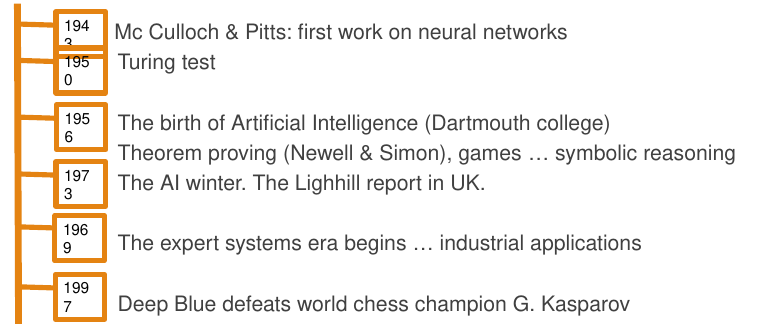
\includegraphics[width=\textwidth]{Images/timeline}
    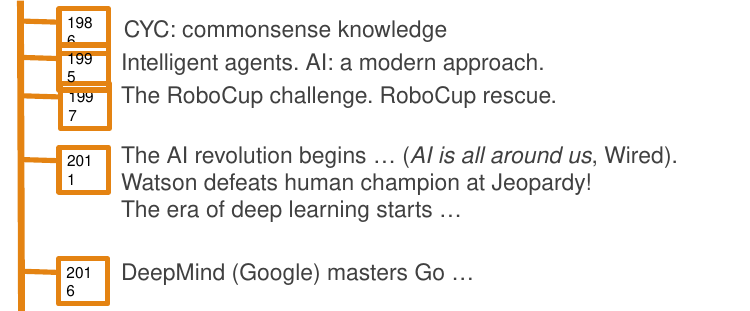
\includegraphics[width=\textwidth]{Images/timeline2}
\end{figure}
The major discover happened on $2020$ are the following:
\begin{description}
    \item [GPT3 (Generative Pre-trained Transformer): ] produced by OpenAI in May $2020$, is 
           a larger and richer language model consisting in $175$ billion machine learning parameters
           used for automatic text generation, translation, user interface synthesis
    \item [DARPA challenge (AlphaDogFights)] with simulated F-16 Air Fighters where on $18-20$ August $2020$
           there was the final Event, where AI system was against each other and the winner was a system by 
           Heron system, that was also able to defeated a human expert top gun fighter $5-0$.
\end{description}
On \cite{andrewNg} Andrew NG says that AI will transform many industries, but it’s not magic and 
almost all of AI’s recent progress is based on one type of AI, in which some input data $(A)$ is used to
quickly generate some simple response $(B)$ [$A \to B$].\newline
Also Andrew Ng says that if a typical person can do a mental task with less than one second of thought,
we can probably automate it using AI either now or in the near future.\newline
Choosing A and B creatively has already revolutionized many industries, it is poised to
revolutionize many more.

ML systems are not (yet?) able to justify in human terms their results, so for some application it is essential
the human knowledge to be able to generate explanations, infact some regulations requires the right
to an explanation in decision-making, and seek to prevent discrimination based on race, opinions,
health, sex and so on, like GPDR.\newline
ML systems learn what’s in the data, without understanding what's true or false, real or imaginary, 
fair or unfair and so it is possible to develop bad/unfair models.

The goal of building AI systems is far from being solved and is still quite challenging in its own.
Building complex AI systems requires the combination of several techniques and approaches, not only ML.\newline
One of the most challenging tasks ahead of us is integration of
perception and reasoning in AI systems.

AI fundamentals is mostly about “Slow thinking” or “Reasoning” and AI fundamentals has the role,
within the AI curriculum, of teaching you about the foundations of a discipline which is now 60 year old.\newline
We will cover different approaches, also some coming of the “Good Old-
Fashioned Artificial Intelligence” (GOFAI) or symbolic AI.

\begin{defi}
Symbolic AI is an high-level "symbolic" (human-readable) representations of problems, the 
general paradigm of searching for a solution, knowledge representation and reasoning, planning.\newline
Symbolic AI was the dominant paradigm of AI research from the mid 1950s until the late 1980s and 
central to the building of AI systems is the \emph{Physical symbol systems hypothesis}, formulated by Newell and Simon.
\end{defi}

The approach is based on the assumption that many aspects of intelligence can be achieved by the 
manipulation of symbols (the physical symbol system hypothesis):
\begin{defi}
A physical symbol system has the necessary and sufficient means for general intelligent action
\end{defi}%CITE WHO SAYS THAT
Human thinking is a kind of symbol manipulation system (a symbol system is necessary for intelligence) and 
machines can be intelligent (a symbol system is sufficient for intelligence).\newline
The hypothesis cannot be proven, we can only collect empirical evidence and observations and experiments
on human behavior in tasks requiring intelligence.

We have two different typologies of AI, that was introduced and considered:
\begin{description}
    \item [Strong AI: ] relies on the strong assumption that human intelligence can be reproduced
                        in all its aspects (general A.I.).\newline
                        It includes adaptivity, learning, consciousness and not only pre-programmed behavior.
    \item [Weak AI: ]   simulation of human-like behavior, without effective thinking/understanding and 
                        no claim that it works like human mind; it is the dominant approach today.
\end{description}
A problem of AI is that computer can't have needs, cravings or desires and Abraham Maslow's define 
a hierarchy of human needs:
\begin{enumerate}
    \item Biological needs (food, sleep, sex, ...)
    \item Safety, protection from environment
    \item Love and belonging, friendship
    \item Self esteem and respect from others
    \item Self-actualization
\end{enumerate}

      \chapter{Search Engine}
An \emph{search engine} it comes of several components that can be viewed in figure \ref{img:searchEngine},
we will start talking about crawling and then we will introduce the other components.

In figure \ref{img:bowTie} there is a bow tie that exploits some consideration about crawler where
we can see that web pages that search engine consider are a small amount of all pages. 

\section{Crawling}
Crawling is a graph visit of the web graph, run 24h each days, in order to discover new web pages and we 
have a direct graph $G = (N, E)$ with $N$ that indicate $N$ changes in nodes (usually trillion of nodes) and
$E$ indicate a link between two nodes.

In crawling we have to choose between several issues:
\begin{itemize}
    \item How to crawl? we can choose between quality ("Best" pages first), efficiency (Avoid duplication) and also 
          about malicious pages (Spam pages, Spider traps) including dynamically generated.
    \item How much to crawl and thus index? Coverage and Relative Coverage (coverage comparated with competitor)
    \item How often to crawl? Freshness: How much has changed?
\end{itemize}
Actually is difficult to decide how to implement and design a crawler that should respect the issues that we have
introduced before.

In figure \ref{img:crawler} it is possible to note the general structure of crawler process, in figure \ref{img:crawlerElement} it 
possible to note the component used to implement a crawler and in the end in figure \ref{img:crawlerAlgorithm} there is an pseudocode 
implementation of Crawler's component.

\begin{figure}
    \caption {Diagramm of Crawler operation}
    \label{img:crawler}
    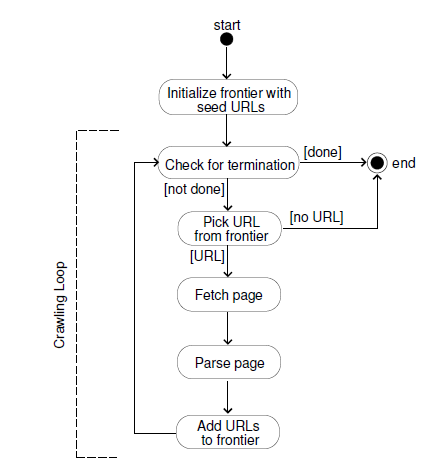
\includegraphics[width=\textwidth]{Images/crawler}
\end{figure}

\begin{figure}
    \caption{Component of Crawler}
    \label{img:crawlerElement}
    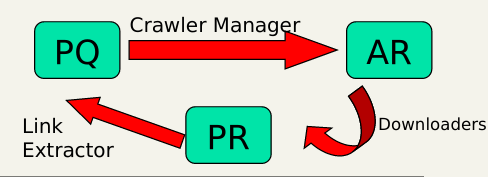
\includegraphics[width=\textwidth]{Images/crawlerComponents}
\end{figure}

\begin{figure}
    \caption{Pseudocode of Crawler components}
    \label{img:crawlerALgorithm}
    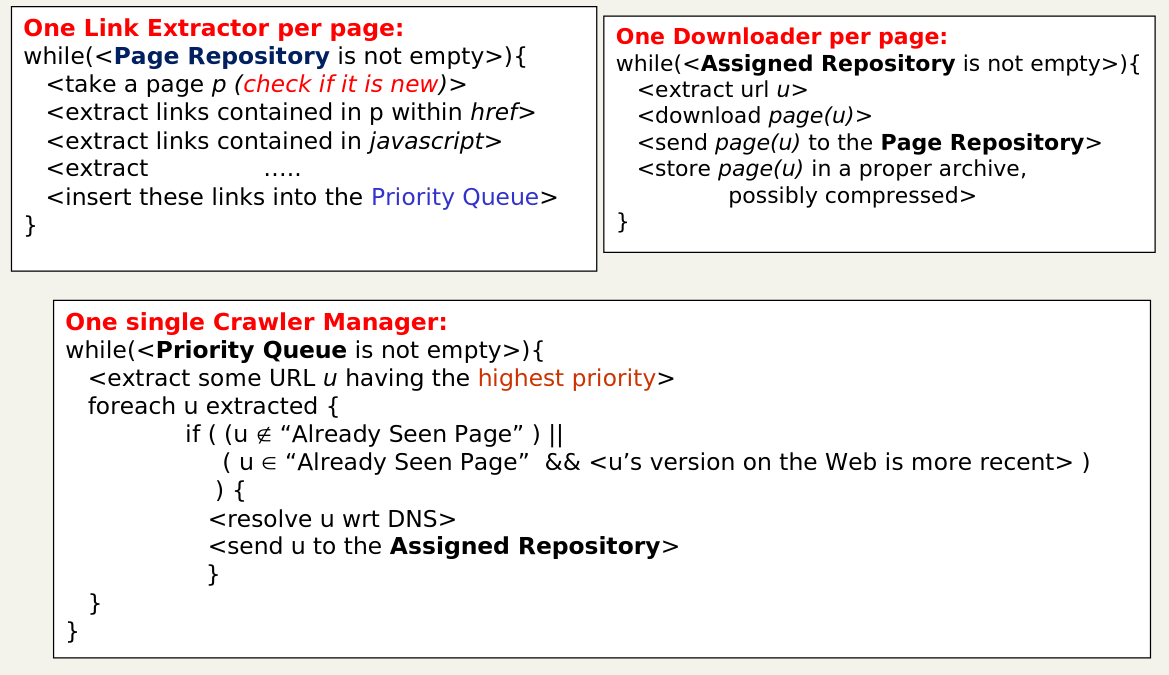
\includegraphics[width=\textwidth]{Images/crawlerPseudocode}
\end{figure}
In visiting the URL frontier we have to define how "good" a page is and there exists several metrics (BFS, DFS, RANDOM, PAGERANK and so on) and also now
we will introduce \emph{Mercator}, an example of search engine released in $1999$, where are present $3$ assumpionts:
\begin{enumerate}
    \item Only one connection per host is open at a time.
    \item a waiting time of a few seconds occurs between successive requests to the same host.
    \item high-priority pages are crawled preferentially.
\end{enumerate}
The structure of Mercator can be viewed in figure \ref{img:mercator} and we have that \emph{Front queues} manage prioritization: prioritizer assigns to an URL an integer priority (refresh,
quality, application specific) between $1$ and $K$ and appends URL to corresponding queue, according to priority.\newline
\emph{Back queues} enforce politeness: each back queue is kept non-empty and contains only URLs from a single host; in a back-queue request it select a front queue randomly, biasing towards higher queues.

\begin{figure}
    \caption{Structure of Mercator search engine}
    \label{img:mercator}
    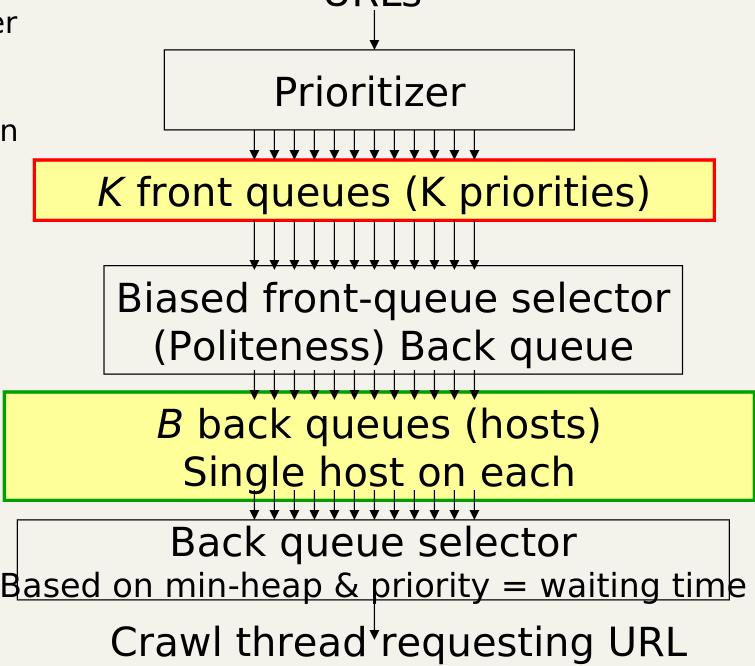
\includegraphics[width=\textwidth]{Images/mercator}
\end{figure}
The \emph{min-heap} contains one entry per back queue and the entry is the earliest time $t_e$ at which the host corresponding to the back queue can be “hit again”:
this earliest time is determined from last access to that host and any time buffer heuristic we choose.\newline
The \emph{crawl thread} consist that a crawler seeks a URL to crawl: extracts the root of the heap, waits the indicate time $t_{url}$, parses URL and adds its out-links to the Front queues.\newline
If back queue $q$ gets empty, pulls a URL $v$ from some front queue (more prob for higher queues): if there’s already a back queue for v’s host, append v to it and 
repeat until q gets not empty, else make q the back queue for v’s host.\newline
If back queue q is non-empty, pick URL and add it to the min-heap with $priority = waiting time t_{url}$.

To check if the page has been parsed/downloaded before URL match, duplicate document match and near-duplicate document match we have several solutions:
\begin{itemize}
    \item Hashing on URLs: after $50$ bln pages, we have “seen” over $500$ bln URLs and each URL is at least $1000$ bytes on average so in overall we have about $500.000 Tb (=500 Pb)$ for just the URLS
    \item Disk access with caching (e.g. Altavista): $>5$ ms per URL check and $>5 ms * 5 * 10^{11}$ URL-checks ($80 years/1PC$ or $30gg/1000 PCs$).
    \item \emph{Bloom Filter} (Archive): for $500$ bln URLs we have about $500 Tbit = 50Tb$
\end{itemize}

\section{Bloom Filter}
An empty Bloom filter is a bit array of $m$ bits, all set to $0$ and there must also be $k$ different hash functions defined, each of which maps or hashes some set element to one of the
$m$ array positions, generating a uniform random distribution.\newline
Typically, $k$ is a small constant which depends on the desired false error rate $\epsilon$, while $m$ is proportional to $k$ and the number of elements to be added and 
to add an element, feed it to each of the $k$ hash functions to get $k$ array positions and set the bits at all these positions to $1$.

To query for an element (test whether it is in the set), feed it to each of the $k$ hash functions to get $k$ array positions and if any of the bits at these positions is $0$,
the element is definitely not in the set; if it were, then all the bits would have been set to $1$ when it was inserted and if all are $1$, then either the element is in the set,
or the bits have by chance been set to $1$ during the insertion of other elements, resulting in a false positive.

In a simple Bloom filter, there is no way to distinguish between the two cases, but more advanced techniques can address this problem and 
the requirement of designing $k$ different independent hash functions can be prohibitive for large $k$, so for a good hash function with a wide output,
there should be little if any correlation between different bit-fields of such a hash, so this type of hash can be used to generate multiple "different" hash functions
by slicing its output into multiple bit fields.\newline
Alternatively, one can pass $k$ different initial values (such as $0, 1, \dots, k-1)$ to a hash function that takes an initial value, or add (or append) these values to the key. 

Removing an element from this simple Bloom filter is impossible because there is no way to tell which of the k bits it maps to should be cleared and although setting any one of those
$k$ bits to zero suffices to remove the element, it would also remove any other elements that happen to map onto that bit, so since the simple algorithm provides no way
to determine whether any other elements have been added that affect the bits for the element to be removed, clearing any of the bits would introduce the possibility of false negatives.

One-time removal of an element from a Bloom filter can be simulated by having a second Bloom filter that contains items that have been removed, however, false positives
in the second filter become false negatives in the composite filter, which may be undesirable and in this approach re-adding a previously removed item is not possible,
as one would have to remove it from the "removed" filter.

Assume that a hash function selects each array position with equal probability, so if $m$ is the number of bits in the array, the probability that a certain bit
is not set to $1$ by a certain hash function during the insertion of an element is
\[ 1 - \frac{1}{m} \]
so if $k$ is the number of hash functions and each has no significant correlation between each other, then the probability that the bit is not set to 1 by any of the hash functions is
\[ (1 - \frac{1}{m})^k \]
and using the well-known identity for $e$ we can obtain for large $m$
\[ (1 - \frac{1}{m})^k = ((1 - \frac{1}{m})^m)^{k/m} \approx -e^{k/m} \]
If we have inserted n elements, the probability that a certain bit is still $0$ is 
\[ (1 - \frac{1}{m})^{kn} \approx -e^{kn}{m} = 0.62^{m/n}\]
It minimize prob. error for $k = (m/n) ln 2$and it is advantageous when $(m/n) << (\text{ key-length in bits } + \log n)$

Pattern maching is a set of objects, whose keys are complex and time costly to be compared (URLs, matrices, MP3 and so on) so we use Bloom Filter to
reduce the explicit comparison and it is effective in hierarchical memories (Example on Dictionary matching).

Another example is \emph{Set intersection}, where we have two machines $M_A$ and $M_B$, each storing a set of items $A$ and $B$ and we wish compute $A \cup B$
exchanging small number of bits.\newline
A solution consist to compute $B - A$ by exchanging small amount of bits ($|A| \log \log |B|$), time depending on $B - A$ and with only $1$ communication round and we consider now
\emph{Patricia Tree}, a special variant of the radix binary trie, in which rather than explicitly store every bit of every key, the nodes store only the position of the first bit
which differentiates two sub-trees.\newline
During traversal the algorithm examines the indexed bit of the search key and chooses the left or right sub-tree as appropriate, and an example can be viewed in figure \ref{img:patricia}.

\begin{figure}
	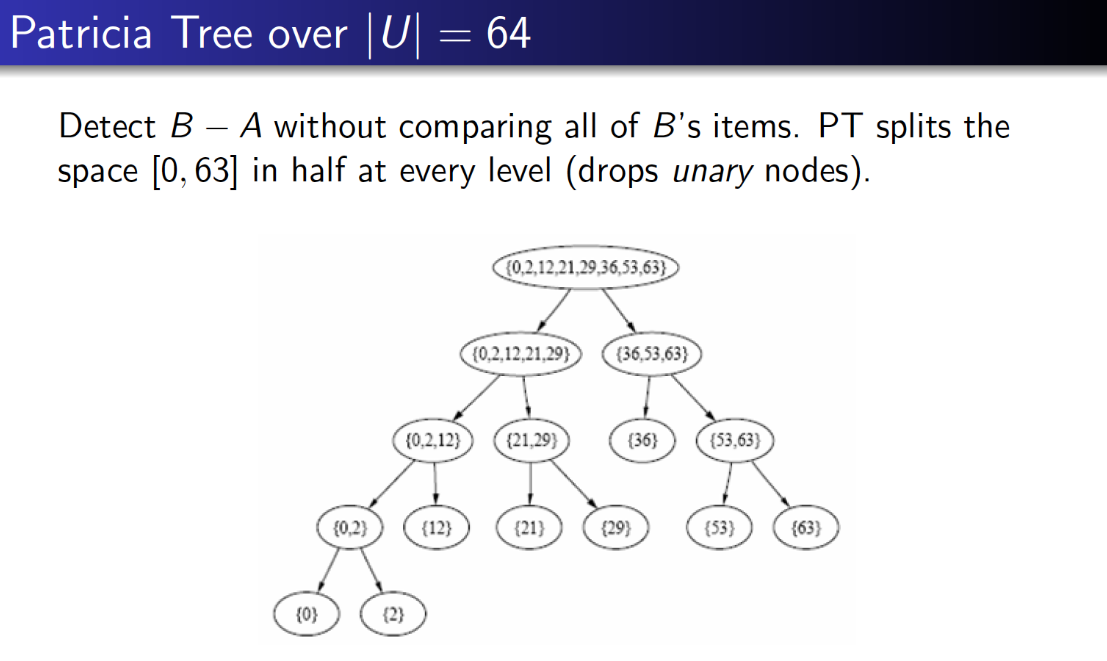
\includegraphics[width=\textwidth]{Images/patricia}
	\caption {Example of Patricia Tree}
	\label{img:patricia}
\end{figure}
Given $PT_A$ and $PT_B$ at machine $M_B$ we procede as follows:
\begin{enumerate}
    \item Visit $PT_B$ top down and compare a node of $PT_B$ against the correspective node in $PT_A$.
    \item If there is a match, the visit backtracks, otherwise proceeds to all children.
    \item If we reach a leaf, then the correspective of $B$ is declared to be in $B - A$
\end{enumerate}
In figure \ref{img:merkleTree} is possible to note Merkle Tree, that are Patricia Tree with hashing and we consider an approximate algorithms, visible in figure \ref{img:approximateAlg},
that use $BF(MT_A)$ to send $MT_A$ in less bits and bookkeeping for its structure, but this of course introduce false-positive errors.
\begin{figure}
	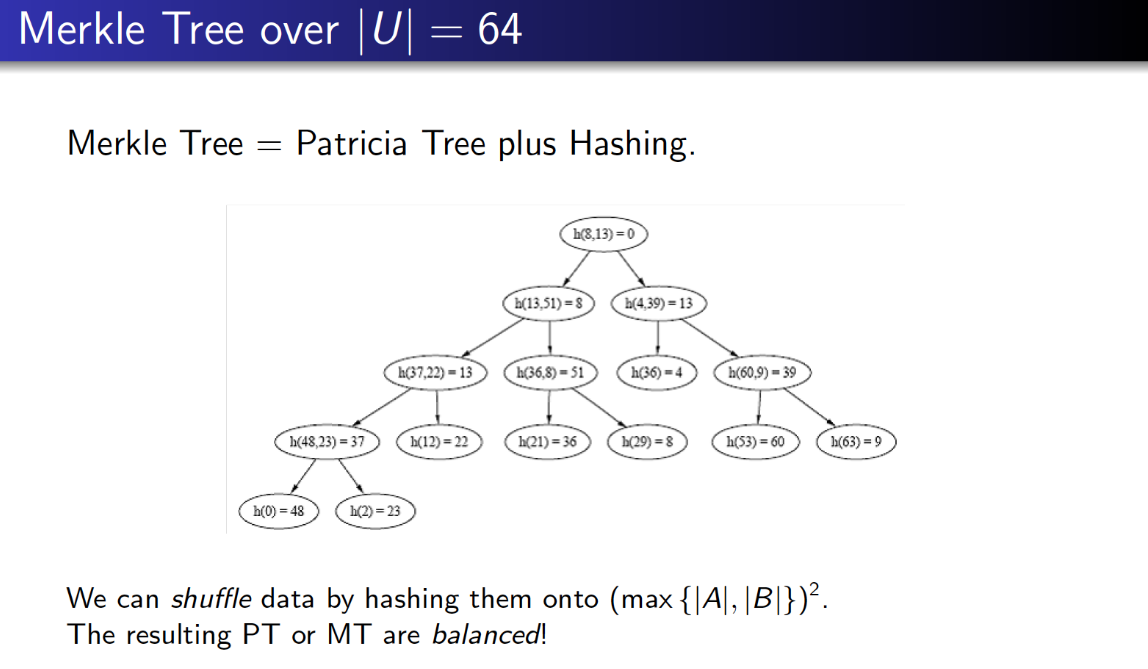
\includegraphics[width=\textwidth]{Images/merkle}
	\caption{Example of Merkle Tree}
	\label{img:merkleTree}
\end{figure}

\begin{figure}
	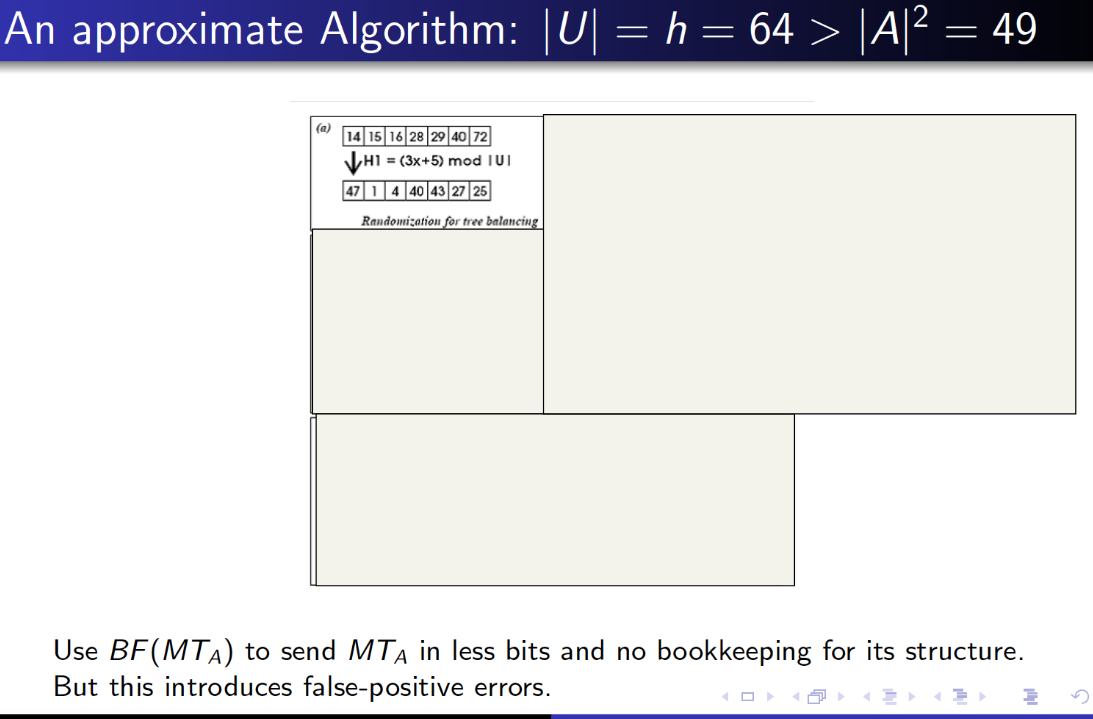
\includegraphics[width=\textwidth]{Images/approximativeAlg}
	\caption{Approximative algorithm to compute Set intersection}
	\label{img:approximateAlg}
\end{figure}
Given $BF(MT_A)$ and $MT_B$, the machine $M_B$ proceeds as follows:
\begin{enumerate}
	\item Visit $MT_B$ top-down and, for each node, check its hash in $BF(MT_A)$.
	\item IF there is a match the visit backtrack, otherwise proceeds to their children.
	\item If we reach a leaf, then the correspective of $B$ is declared to be in $B - A$
\end{enumerate}
Let $m_A = \Theta(|A| \log \log |B|)$ and the optimal $k_A = \Theta(\log \log |B|)$ we send $m_A$ bits for the $BF(A)$ and we have
\[ \epsilon_A = (1/2)^{k_A} = O(1/ \log |B|) \] 
that is the error of $BF(A)$.\newline
The probability of a success for a leaf is given by $(1 - \epsilon_A)^d = \Theta(1)$ and for a correct leaf we have visited its downward path of length $\Theta(\log |B|)$ 
computing $\Theta(\log \log |B|)$ hash functions per node.\newline
This needs a round, $O(|A| \log \log |B|)$ bits, and $O(B - A \log |B| \log \log |B|)$ of reconciliation time.

\subsection{Spectral Bloom Filter}
    We define now an evolution of Bloom Filter, used not only in URL match, with the following definition
    \begin{defi}[Spectral Bloom Filter]
         We have a multiset $M = (S, f_X)$ where $S$ is a multiset and $f_X$ is a count function that return the number of occurrences of $x$ in $M$
    \end{defi}
    Comparated with Bloom Filter we have an slightly large usage of space, but we achieve better performance, and also can be built incrementally for streaming data.

    Applications of this data structure is to answer to two common query:
    \begin{description}
        \item [Iceberg query: ] given $x$ check if $f_X > T$, where $T$ is a dynamically threshold
	\item [Aggregate query: ] $SELECT count(a1) FROM R WHERE a1 = v$
    \end{description}
    B vector is replaced by a vector of counters $C_1, C_2, \dots, C_m$, where $C_i$ is the sum of $f_X$ values for elements $x \in S$ mapping to $i$, and approximations of $f_X$ are stored 
    into $C_{h_1(x)}, C_{h_2(x)}, \dots, C_{h_k(x)}$, but due to conflicts $C_i$ provide only an approximation.

    In figure \ref{img:approximation} is possible to note what is good approximation or a bad approximation of $f_X$, and insertion and deletion are quite simple because we have only
    to increase/decrease each counter by $1$, instead the search operation return the minimum selection (MS) value defined as 
    \[ m_X = \min \{C_{h_1(x)}, \dots, C_{h_k(x)}\} \]

    \begin{figure}
	\caption{Example of approximation between $C_i$ and $f_X$}
	\label{img:approximation}
	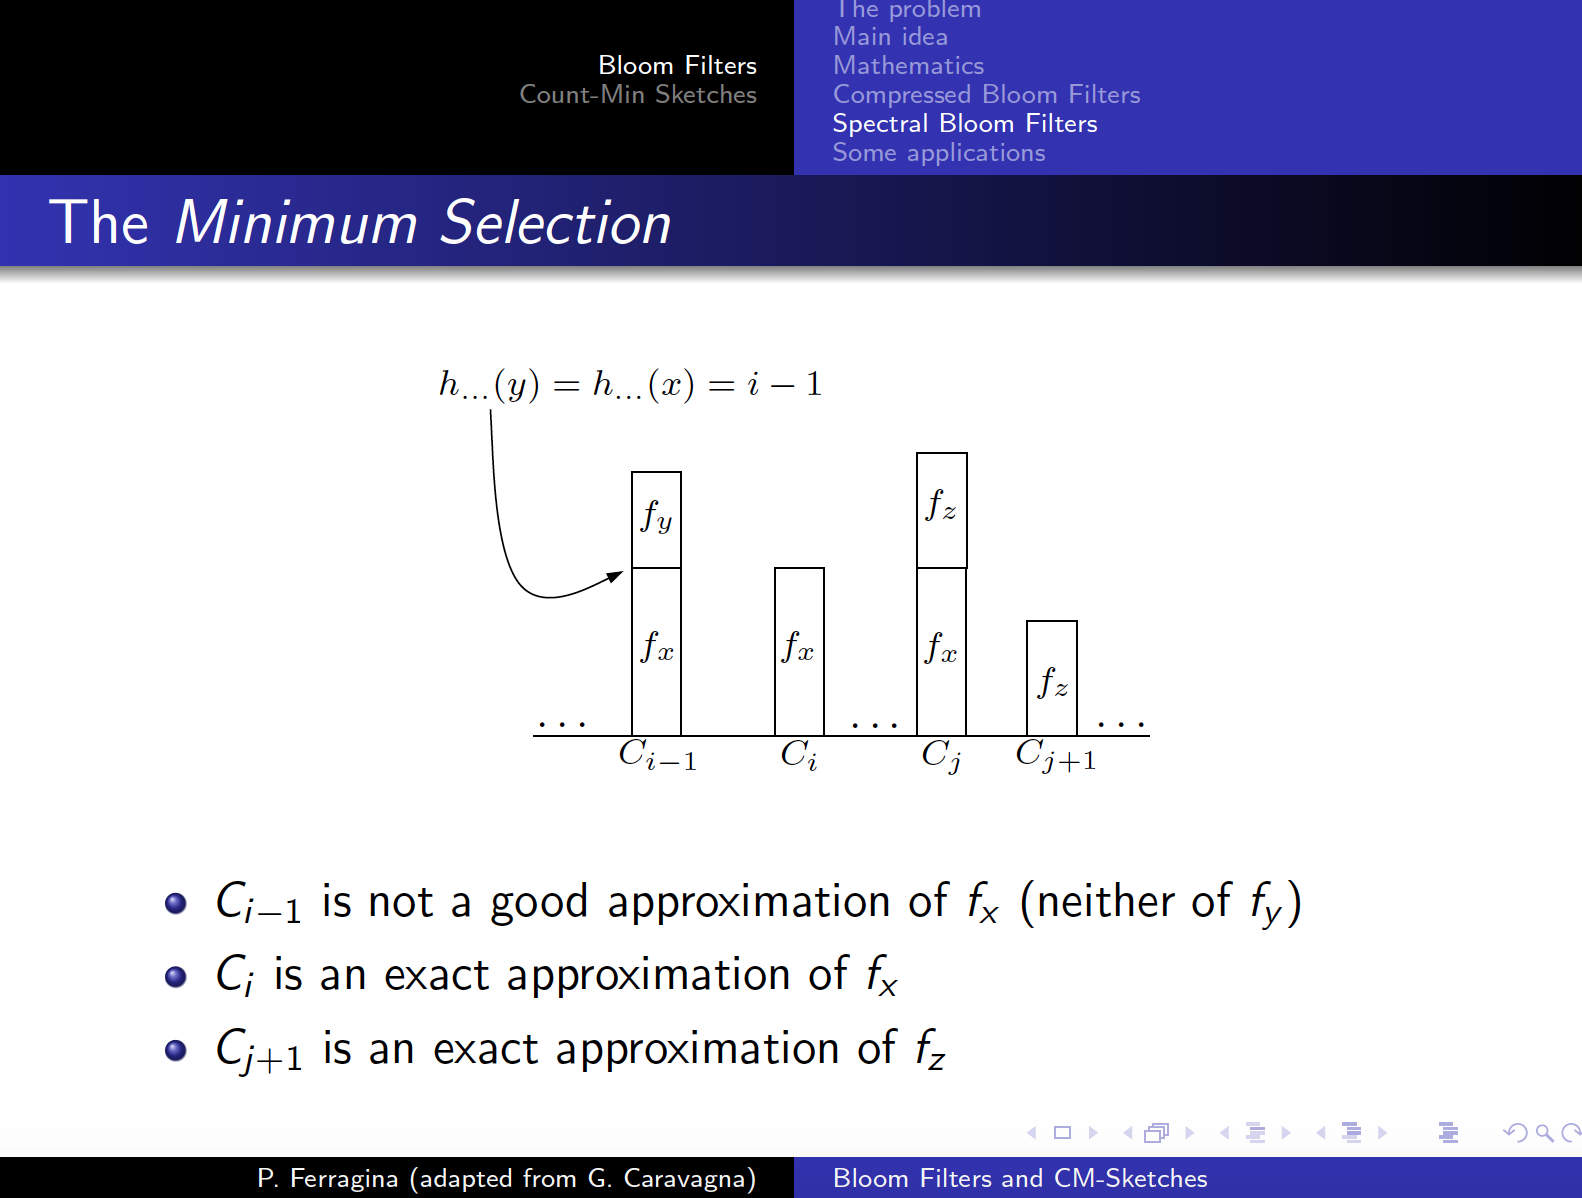
\includegraphics[width=\textwidth]{Images/approximation}
    \end{figure}

    The error rate is the same as bloom filter and we will now prove it 
    \begin{thm}
	For all $x$ it is $f_X \leq m_X$ and we have $f_X \neq m_X$ with probability $E_{SBF} = \epsilon \sim (1-p)^k$
    \end{thm}
    \begin{proof}
	The case that $m_X < f_X$ can not even happen instead the case $m_X > f_X$ happen when all the counter have a collision, that correspond to the event of a false positive in Bloom Filter
    \end{proof}
    Mainly we have two challenges: allow insertion/deletion while we keeping low $E_{SBF}$ and dynamic array of variable-length counters and to solve the first problem we will use \emph{Recurring Minimum (RM)} that is defined as 
    \begin{defi}
	An element has a RM iff more than one of its counters has value equal to the minimum
    \end{defi}
    An item which is subject to a Bloom Error is typically less likely to have recurring minimum among its counters, because we have the following basic idea, using two SBF:
    \begin{enumerate}
	\item For item $x$ with RM we use $m_X$ as estimator, which is highly probable to be correct and hence $E_{SBF_1} < \epsilon$
	\item For items with a SM we use a secondary SBF which is $|SBF_2| << |SBF_1|$ and thus can guarantee $E_{SBF_2} << \epsilon$.
    \end{enumerate}
    With this approach we use more space which could be used for enlarging the single BF, but experiments show that improvements may be remarkable.

    The insertion handles potential future errors, because we increase all counters of $x$ in $SBF_1$ and if $x$ has a $SM$ in $SBF_1$ we look for $x$ in $SBF_2$ and 
    if yes we increase all counters of $x$ in $SBF_2$, otherwise we set $x$ in $SBF_2$ to be the minimum value in $SBF_1$.

    The deletion is the inverse of insertion, so we decrease all counters of $x$ in $SBF_1$ and if $x$ has a SM in $SBF_1$ we decrease all counters of $x$ in $SBF_2$.

    In lookup we have that if $x$ has a RM in $SBF_1$ we return it otherwise we set $m_x^2$ as the value of $x$ in $SBF_2$ that if it is $> 0$ we return it otherwise we return the min value of $x$ in $SBF_1$.


\section{Parallel Crawlers}
    Web is too big to be crawled by a single crawler, work should be divided avoiding duplication so we need several crawlers that works in parallel and assignment 
    between different crawlers can be done in two ways:
    \begin{description}
	    \item [Dynamic assignment: ] central coordinator dynamically assigns URLs to crawlers and it needs communication between coordinator/crawl threads.
	    \item [Static assignment: ] web is statically partitioned and assigned to crawlers and crawler only crawls its part of the web, no need of coordinator and thus communication
    \end{description}
    The Dynamic assignment is problematic because it is computationally expensive and may be complicated, anyway also static assignment has two problem:
    \begin{itemize}
	\item Load balancing the number of URL assigned to crawler because static schemas based on hosts may fail and dynamic assignment may be complicated
	\item Managing the fault-tolerance so in case we have a death of crawler or we have a new crawler we have to recompete the hash function and choose which crawler to assign.
    \end{itemize}
    A nice technique to solve this problem consist in \emph{consistent hashing}, a tool for Spidering, Web Cache, P2P, Routers Load Balance and Distributed FS.\newline
    It consist that item and servers are mapped to unit circle via hash function ID() and item $K$ are assigned to first server $N$ such that $ID(N) \geq ID(K)$, as we can 
    see in figure \ref{img:consistentHashing}.\newline
    Each server gets replicated $\log S$ times, adding a new server moves points between an old server to the new one, only, we have that in average a server gets $\frac{n}{s}$ element.

    \begin{figure}
	\caption{Consistent Hashing Example}
	\label{img:consistenHashing}
	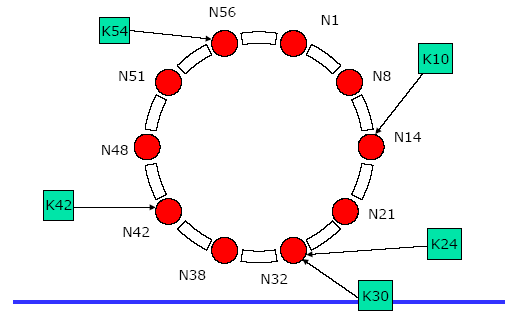
\includegraphics[width=\textwidth]{Images/consistentHashing}
    \end{figure}


\section{Compressed storage of Web Graph}
    Given a directed graph $G = (V, E)$, where $V$ are URLs and $E = (u, v)$ if $u$ has an hyperlink to $v$, also isolated URLs are ignored (they do not have IN and/or OUT)
    and we have three key properties:
    \begin{description}
	    \item [Skewed distribution: ] probability that a node has $x$ links is $1/x^{\alpha}$ with $\alpha \approx 2.1$, so in-value degree follows power law distribution, 
		    			  as we can see in figure \ref{img:altavistaCrawl} and \ref{img:webbaseCrawl}.

					  \begin{figure}
						  \caption{In-degree value in Altavista Crawl in 1997}
						  \label{img:altavistaCrawl}
						  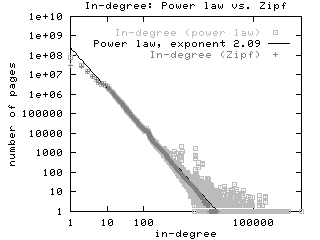
\includegraphics[width=\textwidth]{Images/altavistaCrawl}
					  \end{figure}

					  \begin{figure}
						  \caption{In-degree value in WebBase crawl in 2001}
						  \label{img:webbaseCrawl}
						  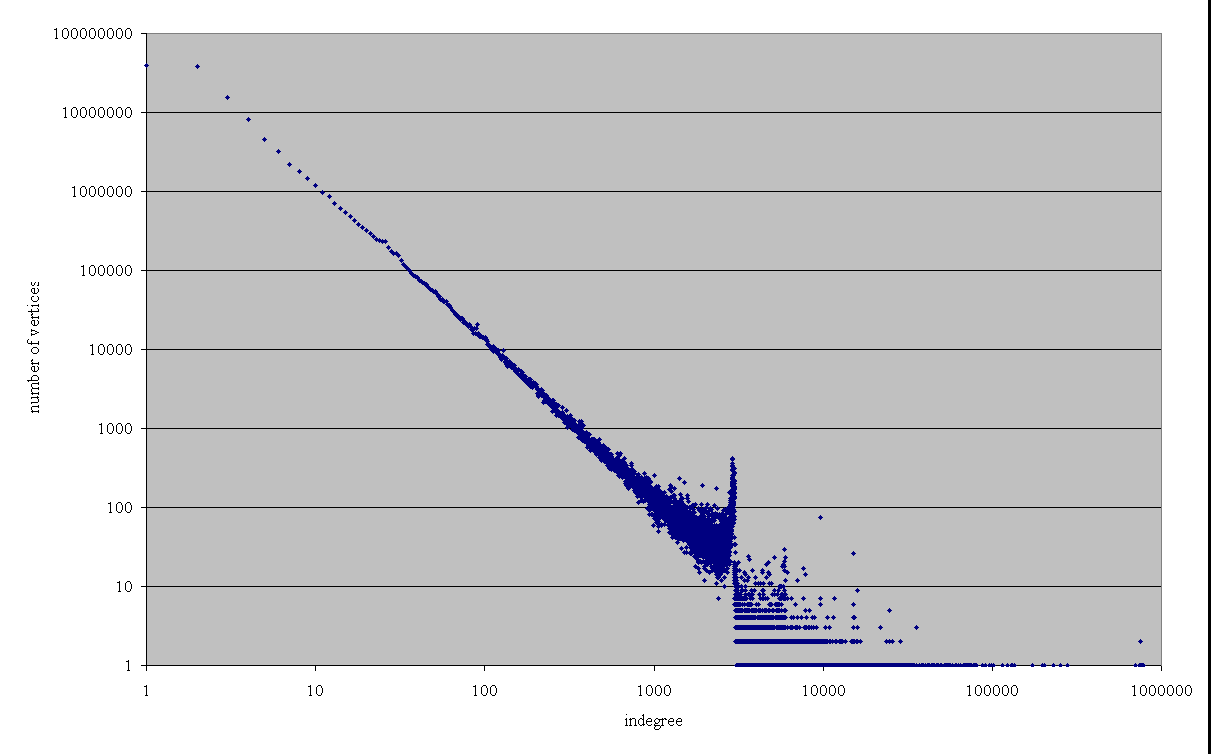
\includegraphics[width=\textwidth]{Images/webBaseCrawl}
					  \end{figure}
						  
	    \item [Locality: ] usually, most of the hyperlinks from URL $u$ point to other URLs that are in the same host of $u$ (about $80\%$), so hosts in the same domain are 
		               close to each other in the lexicographically sorted order, and thus they get close docIDs.

	    \item [Similarity: ] if URLs $u$ and $v$ are close in lexicographic order, then they tend to share many hyperlinks, so we have that each bit of the copy list informs 
		                 whether the corresponding successor of $y$ is also a successor of the reference $x$ and the reference index is the one in $[0, W]$ that gives the best compression,
				 as we can see in figure \ref{img:copyList}.

				 \begin{figure}
					\caption{Example of Copy List}
					\label{img:copyList}
					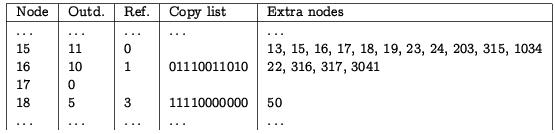
\includegraphics[width=\textwidth]{Images/compressedAdjancency}
				 \end{figure} 
    \end{description}
    To consider these properties we now introduce \emph{copy lists}, to compress information and exploits locality and similarity, but also consider the \emph{copy block}, 
    visible in figure \ref{img:copyBlock}, where the first bit specifies the first copy block and last block is omitted because we know the length from $Out_d$.

    \begin{figure}
	\caption{Example of Copy Block}
	\label{img:copyBlock}
	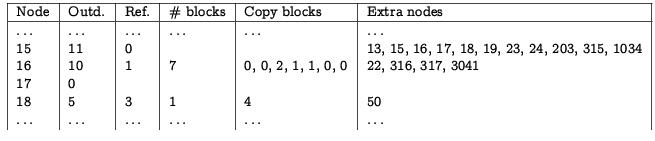
\includegraphics[width=\textwidth]{Images/copyBlock}
    \end{figure}

\section{Locality-sensitive hashing and its applications}
    Given $U$ users, described with a set of d features, the goal is to find (the largest) group of similar users, and to find these group we have three approaches:
    \begin{enumerate}
	\item Try all groups of users and, for each group, check the (average) similarity among all its users.\newline
	      The problem of this approach is that it requires $2^U * U^2$ and also if we limit groups to have a size $\leq L$ we have anyway $U^L * L^2$ 
	      that is computationally infeasible with large $U$.

	\item Interpret every user as a point in a $d$-dim space, and then apply a clustering algorithm, where each iterations require $K * U$ and iterations are relatively small.\newline
	      This approach is locally optimal, comparing users/points costs $O(d)$ in time and space and iterate $k = 1, \dots, U$ costs $U^3 < U^L$, that are in order of years, so 
	      in $T$ time we can manage $U = T^{1/3}$ users.
	
	\item Generate a fingerprint for every user that is much shorter than d and allows to transform similarity into equality of fingerprints.\newline
	      It is randomized, correct with high probability and it guarantees local access to data, which is good for speed in disk/distributed setting.

	      We consider two vectors $p, q \in \{0, 1\}^d$ and we define the \emph{hamming distance} $D(p, q)$ as the number of bits where $p$ and $q$ differ;
	      we define also a \emph{similarity} measure as 
	      \[ s(p, q) = s = \frac{d - D(p, q)}{d} \quad 0 \leq s \leq 1 \]
	      We define now hash functions $h$ by choosing a set $l$ of $k$ random coordinates and we have that the propability to $x$ random such that $p(x) = q(x)$ is defined as 
	      \[ P[\text{picking } x \text{ random such that } p(x) = q(x)] = \frac{d - D(p, q)}{d} = s \]
	      The probability that the hash function $h_I$ has the same value in $p$ and $q$ is defined as 
	      \[ P[h_I(p) = h_I(q)] = s^k = (\frac{d - D(p, q)}{d})^k \]
	      In case we have larger $k$ we have small false positive, instead if we have a large $l$ we have small false negative.

	      We can iterate $L$ times the $k$ projections $h_I(p)$ and we set $g(p) = <h_1(p), h_2(p), \dots, h_L(p)>$, so we declare "$p$ matches $q$" if exist a $I$ such that
	      $h_I(p) = h_I(q)$ and we have that probability of a match defined as 
	       \begin{align}
		      P[g(p) \approx g(q)] & = 1 - P(h_{I_j}(p) \neq h_{I_j}(q) \, \forall j) \\
		                           & = 1 - [P(h_{I_j}(p) \neq h_{I_j}(q)]^L \\
					   & = 1 - (1 - s^k)^L 
	      \end{align} 
	      This probability follow the aspect described in figure \ref{img:matchesProb} and we have that we have to scan all $L$ hash function to create a $L$ fingerprint 
	      with a problem in time complexity.

	      To solve this problem we define for every $p_i$ element $g(p_i) = <h_{I_1}(p_i), h_{I_2}(p_i), \dots, h_{I_L}(p_i)>$ and to compute we follow this algorithm
	     \begin{enumerate}
		\item Sort by $I_1$, scan $g(p_i)$ and find group of continuous vector that have the same first component
		\item Sort by $I_2$, scan $g(p_i)$ and find group of continuos vector that have the same second component
		\item Repeat this approach $L$ times until you sort for $I_L$
	     \end{enumerate}
	     This approach is done by offline search engine, where it is possible to compute statistically connected components, instead online search engine, like databases, 
	     given a query $w$ compute $h_{I_1}(w), \dots, h_{I_L}(w)$ and check the vectors in the buckets $h_J(w)$.

	    This approach of LSH(Locality-sensitive hashing) finds correct clusters with high probability, compares only very short (sketch) vectors, does not need to know the number
	    of clusters and sorts $U$ short items, with few scans.

    \end{enumerate}

\section{Document Duplication}
    The web is full of duplicated content, and exist only few exact duplicate documents but many cases of near duplicates docs (differ for Last modified date, malicious, spam and so on)
    so in this section we will analyze how to determine if two document are duplicates.

   To determine an exact duplication there are several approaches:
   \begin{itemize}
	\item Obvious (slow) technique, like \emph{checksum} (no worst-case collision probability guarantees) or \emph{MD5} (cryptographically-secure string hashes)
	\item Karp-Rabin (fast) scheme: it is a \emph{Rolling hash} (split doc in many pieces), it use arithmetic on primes, it is efficient and has other nice properties.\newline
	      We consider an $m$ bit string $A = 1 a_1 \dots a_{m-1} a_m$ and we choose a prime $p$ in the universe $U$, such that $2p$ uses few memory-words (hence $U \approx 2^64$),
	      so we define the fingerprints $f(A) = A \mod p$, that has a nice properties that if $B = 1 a_2 \dots a_{m-1} a_m a_{m+1}$ we have that 
	      \[ f(B) = [2(A - 2^m - a_1 2^{m-1}) + a_{m+1} + 2^m] \mod p \]
	      and the probabilities that we have a false positive is defined as 
	      \[ \begin{cases}
		      P[\text{false hit to } A \text{ and } B \text{ on same window}] & = \text{Probability } p \text{ divides } (A - B) \\
		                                                                      & = \frac{\# div(A - B)}{\#prime(U)} \\
										      & \approx \frac{(\log (A + B)}{\# prime(U)} \\
										      & = \frac{m \log U}{U} 
		 \end{cases} \]
    \end{itemize}
    Now we consider the problem to given a large collection of documents identify the near-duplicate documents and this aspect is important because it has been found that
    in $1997 30\%$ of web-pages was near-duplicates.


    A common approach used is the \emph{shingling}, where from docs we obtain sets of shingles that are a dissection of document in $q-$gram (shingles), with usually $4 \leq q \leq 8$,
    and the near-duplicate document detection problem reduces to set intersection among integers (shingles), but this naive approaches is computationally expensive so we consider now
    a better approach that use the \emph{Jaccard similarity}, defined as 
    \[ sim(S_A, S_B) = \frac{| A \cap B|}{|A \cup B|} \]
    but also this approach has the problem that we have to compute the similarity of both $A$ and $B$, so a solution consist to use the min hashing, where we define a permutation function,
    we apply them and we take the min element in the permutation of $A$ and $B$.\newline
    An heuristic consist to use $200$ random permutation or pick the $200$ smallest item using only a single permutation, so we obtain a $200$ vector per set which we compare using Hamming distance,
    but of course we can choose how many $k$ element to consider to estimate the Jaccard similarity; the importance of this approximation yields to this important proposition, that will stated and proved
    \begin{prop}
	    $P(\alpha, \beta)$ is exactly the Jaccard similarity $JS(S_A, S_B)$
    \end{prop}
    \begin{proof}
	We give the proof in a slightly more general setting: consider a family of sets whose elements are drawn from a common universe and 
	view the sets as columns of a matrix $A$, with one row for each element in the universe.\newline
	The element $a_{ij} = 1$ if element $i$ is present in the set $S_j$ that the $j$th column represents and let $\Pi$ be a random permutation of  the  rows of $A$;
	denote  by $\Pi(S_j)$ the column that results from applying $\Pi$ to the $j$th column and finally, let $x_{\Pi_j}$ be the index of the first row in which the column
	$\Pi(S_j)$ has a $1$, now we prove that $P(\alpha, \beta) = JS(S_A, S_B)$ and if we can prove this, the theorem follows.

	Consider two columns $j_1, j_2$ and the ordered pairs of entries of $S_{j_1}$ and $S_{j_2}$ partition the rows into four types, as we can note in figure \ref{img:jaccardProof},
	denote by $C_{00}$ the number of rows with $0$’s in both columns, $C_{01}$ the second, $C_{10}$ the third and $C_{11}$ the fourth, then 
	\[ JS(S_{j_1}, S_{j_2}) = \frac{C_{11}}{C_{01} + C_{10} + C_{11}} \]
	To complete the proof by showing that the right-hand side equals to $P(x_{j_1}^{\Pi} = x_{j_2}^{\Pi})$, consider scanning columns $j_1,j_2$ in increasing row
	index until the first non-zero entry is found in either column, and because $\Pi$ is a random permutation, the probability that this smallest row
	has a $1$ in both columns is exactly the right-hand side of Equation.
    \end{proof}
    Another important similarity function is the \emph{cosine Similarity} defined as 
    \[ \cos \alpha = \frac{p * q}{||p|| ||q||} \]
    The computation of the scalar product between $p$ and $q$ is huge, so to solve this problem we use an approximation that consist to construct a random hyperplane $r$ of dimension $d$ and unit norm,
    so we define a sketch vector $h_r(p) = sign(p * r) = \pm 1$ and in a similar way we define a sketch vector for $q$ so we have this proposition
    \begin{prop}
	    $P(h_r(p) = h_r(q)) = 1 - \frac{\alpha}{\pi}$ and also $P(h_r(p) \neq h_r(q)) = \text{hyperplane falls between } p \text{ and } q$
    \end{prop}
    With this probabilistic interpretation we have $O(nk)$ time for each scalar product with an overall time of $O(D * n * k)$, instead if we use $sort(D)$ (I/O efficient) 
    we have $O(D^2)$ that do not scale very well.



      \chapter{Index Construction}
In these chapter we will analyze how we construct inverted index and storage in memory/disk, we will consider 
\emph{SPIMI} (Single-pass in-memory indexing) and \emph{Multi-way Merge-sort}, but also distributional caching.

\section{SPIMI approach}
SPIMI is an approach to storage inverted index using a single pass in memory and has two key ideas:
\begin{enumerate}
	\item Generate separate dictionaries for each block of docs (no need for term map to termID)
	\item Accumulate postings in lists as they occur in each block of docs, in internal memory.
\end{enumerate}
With this approach we generate an inverted index for each block, where also compression is possible and 
in figure \ref{img:spimi} there is the pseudocode of SPIMI approach.

\begin{figure}
	\caption{SPIMI pseudocode}
	\label{img:spimi}
	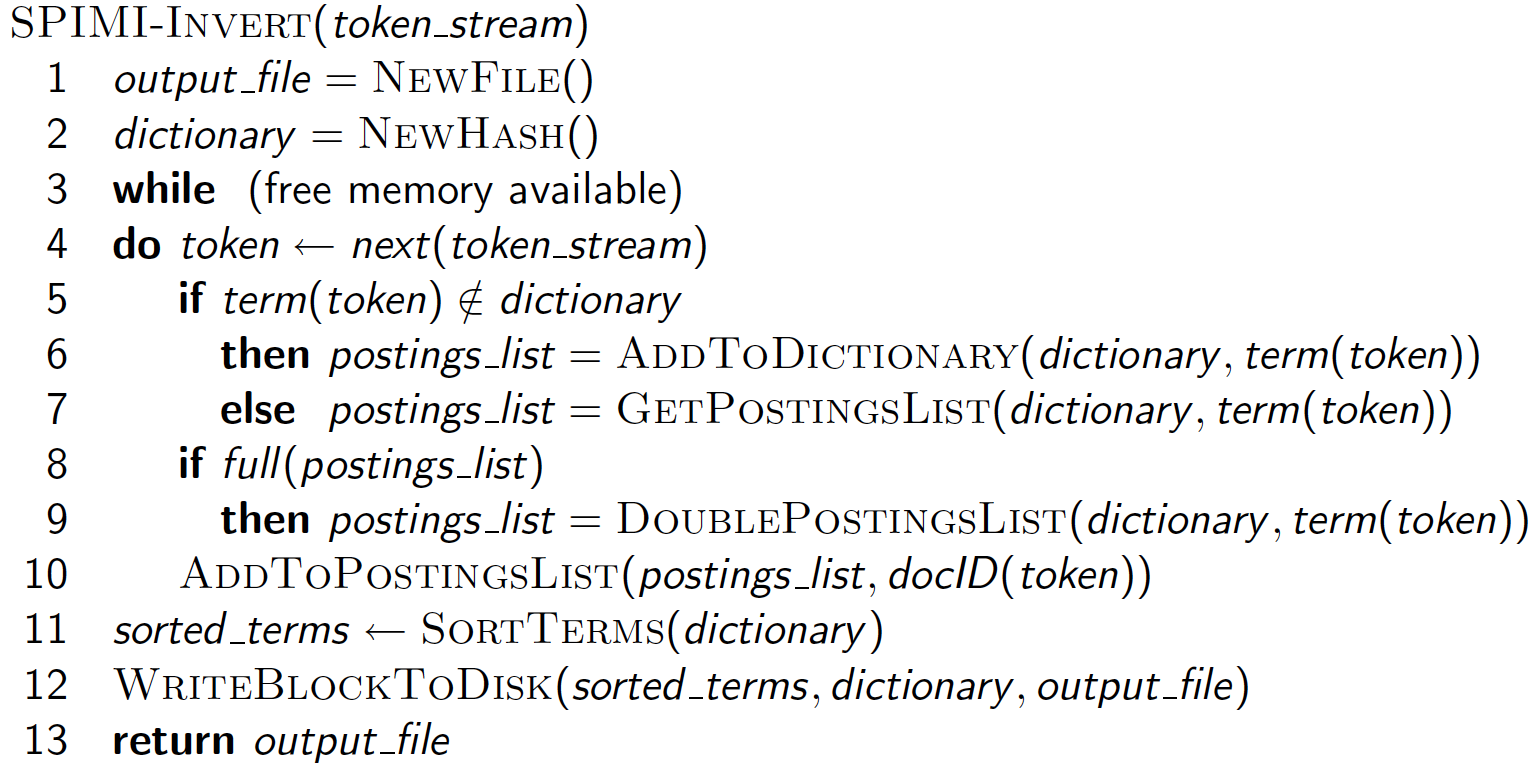
\includegraphics[width=\textwidth]{Images/spimi}
\end{figure}
There are some problems with this approach, like we decide always to double dimension of block when is full, also 
we assign TermID, create pairs $<termID, docID>$ and sort pairs by TermID.

Given a query $q$ we require $N / m$ queries whose results have to be combinated, where $N$ is the number of items 
and $m$ is the dimension of main memory.


To sort $n$ inverted index we accumulate terms, and in a certain time we will encounter again, so we 
assume $|\text{dictionary}| \leq M$ and we have the following steps:
\begin{enumerate}
    \item Scanning and build dictionary of distinct tokens.
    \item Sort the tokens, assign lexicografic IDs such that $T_1 \leq_L T_2 \To ID(T_1) \leq ID(T_2)$
    \item Scan documents and we create pair $<term ID, docID>$.
    \item Sort by first component and then to second component and since the order of terms are 
	  lexicografically sort of first component is this correct.
    \item Decode termID, such that scanning pair in substituting termID with terms, by using the internal
	  memory dictionary.
\end{enumerate}
This sorting is stable, a properties that means that we keep reciprocal order of equal items.

\section{Multi-way merge sort}
We will now consider the multi-way merge-sort, called also \emph{BSBI} (Blocked sort-based Indexing), that consist that
we map term to termID to be kept in memory for construction the pairs and needs two passes, unless we use hashing
and thus with some probability of collision.

This merge-sort consist in particular in two phases:
\begin{enumerate}
    \item Scan input and divide on block of size $M$, where we have for each block $2M/B$ I/Os where $B$ 
	  is the size of block.\newline
	  The total cost of this step is $\frac{2M}{B} * \frac{n}{M} = O(\frac{n}{B})$ I/Os.
    \item Merge $X = M/B-1$ runs, given a $\log_X N/M$ passes, as we can see in figure \ref{img:multiWayMerging}

	  \begin{figure}
	      \caption{Multiway Merge-sort merging}
	      \label{img:multiWayMerging}
	      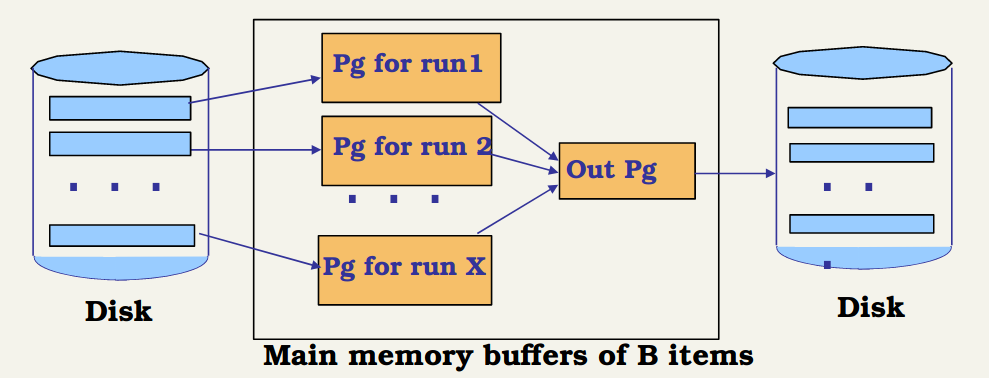
\includegraphics[width=\textwidth]{Images/multiwayMerge}
	  \end{figure}
	  We have to compare $k$ minimum comparison to find the smallest and write in output and in case 
	  output is full we have to flush on memory harddisk/SSD, so we have $O(\frac{X}{B})$ I/Os to find
	  a list of $X$ items in $k$ sorted rows, and we have $\log _k \frac{n}{M}$ levels,
	  yields to a total cost of $O(\frac{n}{B} \log_k \frac{n}{M})$.
\end{enumerate}

\section{Distributed indexing}
For web-scale indexing we must use a distributing computing cluster of inverted index, and since $2004$
Google use \emph{Map Reduce}, that we will introduce later, but we now introduce the distributed indexing.

We maintain a master machine directing the indexing job, considered “safe” and we break up indexing 
into sets of (parallel) tasks, where master machine assigns tasks to idle machines and other machines
can play many roles during the computation.\newline
We will use two sets of parallel tasks, Parsers and Inverters, so we break the document collection in two ways:
\begin{description}
	\item [Term-based partition: ] one machine handles a subrange of terms,
		                       as we can note in figure \ref{img:termBased}.
    \item [Doc-based partition: ] one machine handles a subrange of documents, 
	    			  as we can note in figure \ref{img:docBased}.
\end{description}

\begin{figure}
	\caption{Term-based Distributed indexing}
	\label{img:termBased}
	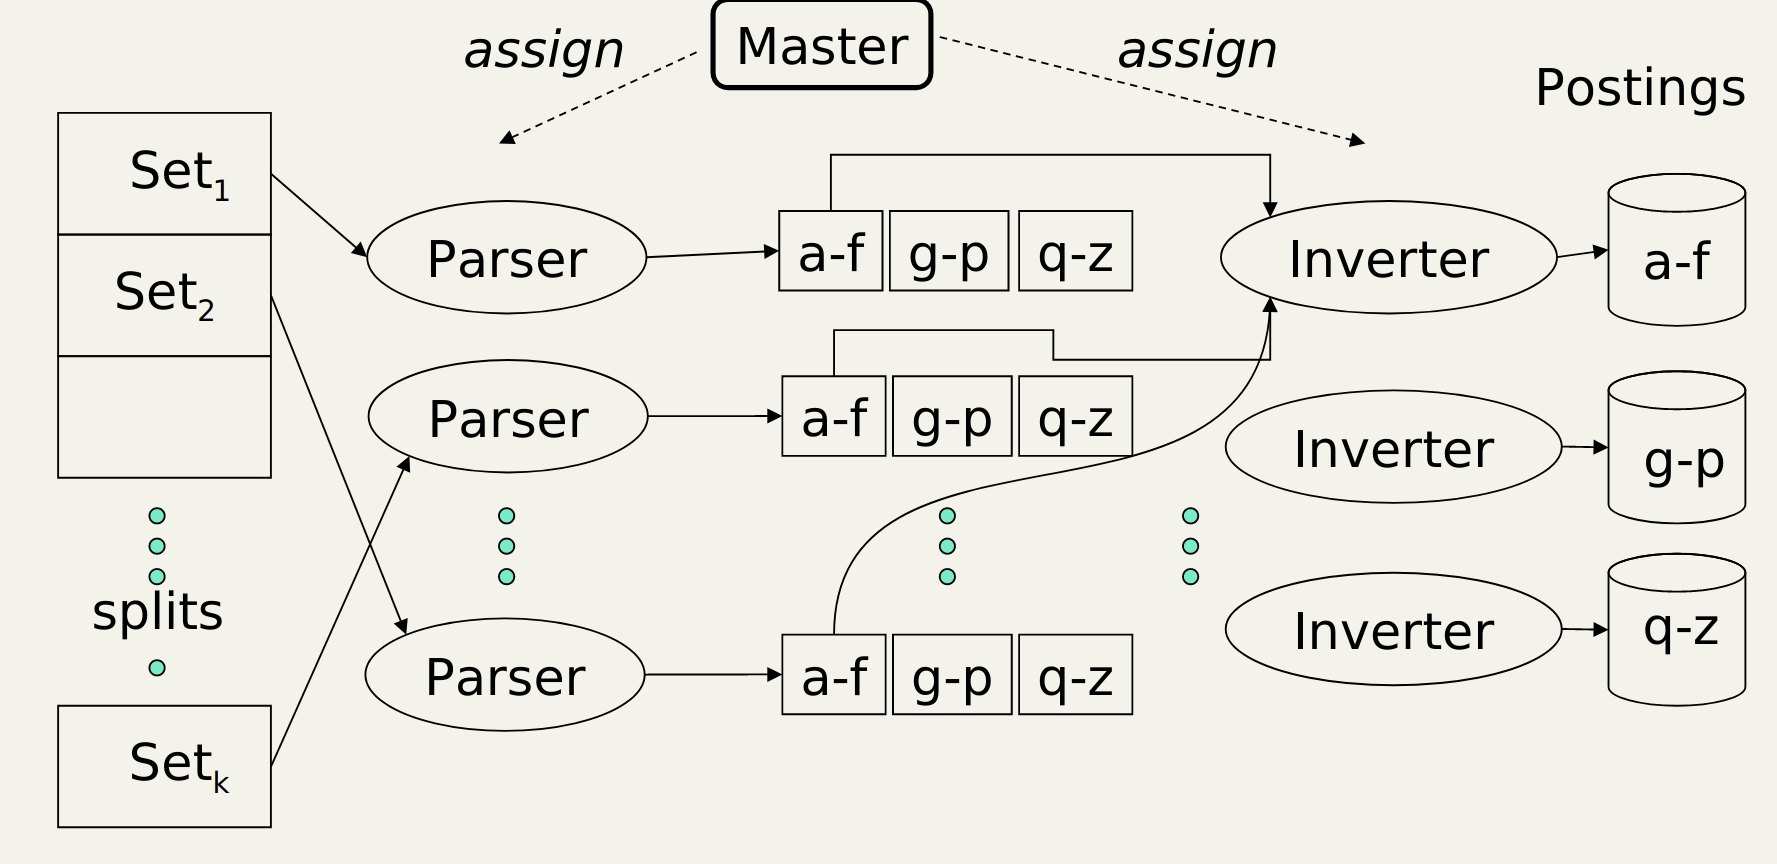
\includegraphics[width=\textwidth]{Images/termBased}
\end{figure}
\begin{figure}
	\caption{Doc-based Distributed indexing}
	\label{img:docBased}
	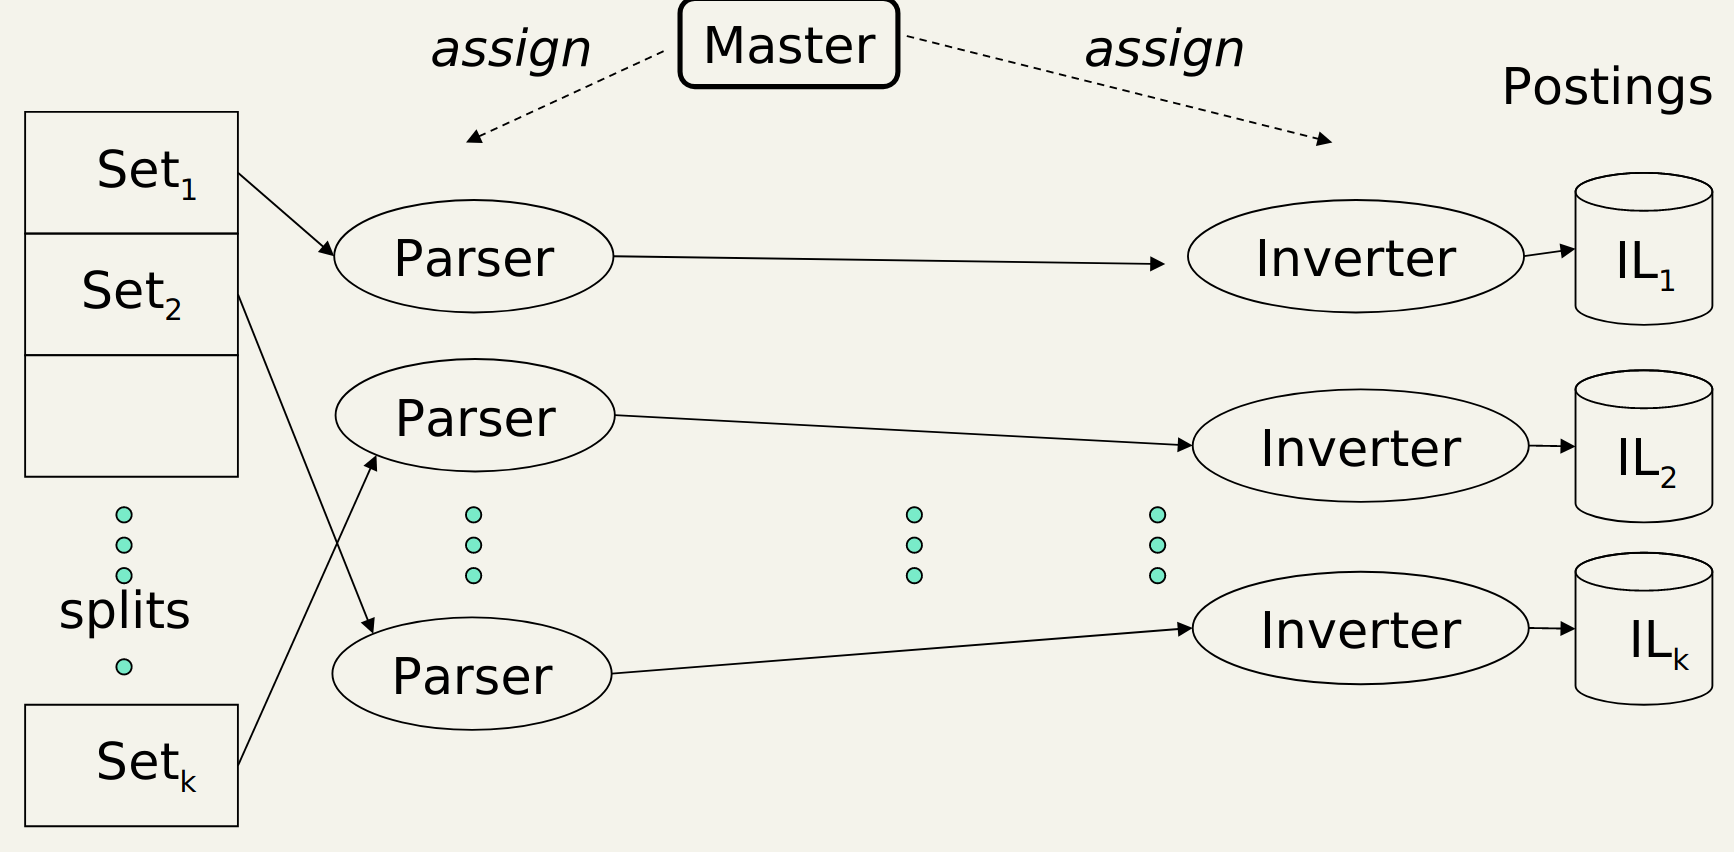
\includegraphics[width=\textwidth]{Images/docBased}
\end{figure}
\emph{MapReduce} is a robust and conceptually simple framework for distributed computing, 
without having to write code for the distribution part and Google indexing system (ca. $2004$) 
consists of a number of phases, each implemented in MapReduce.

Up to now, we have assumed static collections, now more frequently occurs that documents come in over time
and documents are deleted and modified, so this induces postings updates for terms already in dictionary
and new terms added/deleted to/from dictionary.

A first approach is to maintain “big” main index, and new docs go into “small” auxiliary index, where 
we search across both, and merge the results.\newline
In case of deletions we use an invalidation bit-vector for deleted docs, so we filter search results
by the invalidation bit-vector and periodically, we re-index into one main index.

The problem is this approach is that has poor performance: merging of the auxiliary index into the main index
is efficient if we keep a separate file for each postings list and merge is the same as a simple append
[new docIDs are greater] but this needs a lot of files so is inefficient for O/S, anyway
in reality we use a scheme somewhere in between, like split very large postings lists, 
collect postings lists of length $1$ in one file and so on.

We introduce now \emph{Logarithmic merge}, where we maintain a series of indexes, 
each twice as large as the previous one ($M, 2M , 2^2 M, 2^3 M, \dots 2^iM$) and we keep a small index
$Z$ in memory of size $M$ and we store $I_0, I_1, I_2, \dots$ on disk and if $Z$ gets full, 
we write to disk as $I_0$ or merge with $I_0$ (if I0 already exists).\newline
Either write $Z + I0$ to disk as $I_1$ (if no I1) or merge with $I_1$ to form $I_2$, and so on.

Some analysis, with $C = $total collection size) we have that auxiliary and main index has that 
each text participates to at most $(C/M)$ mergings because we have $1$ merge of the two indexes (small and large)
every $M$-size document insertions, instead in logarithmic merge each text participates to no more than
$\log (C/M)$ mergings because at each merge the text moves to a next index and they are at most $\log (C/M)$.

Most search engines now support dynamic indexing (news items, blogs, new topical web pages), 
but (sometimes/typically) they also periodically reconstruct the index, query processing is then
switched to the new index, and the old index is then deleted.


      \chapter{Compression}
In this chapter we will consider how to compress documents, that deal the problem to reduce 
the amount of data that are travel across network.

Snappy is a compression/decompression library that implement it, usable with several language and 
Google has implement recently \emph{Brotli}, a new compression algorithm for internet.

\section{LZ$77$ Compression Method}
LZ$77$ is a compression method, where given a input in the form "past\_string
|string", so LZ$77$ start from string and using past knowledge 
we encode the document with triples of form $<$dist, len, next-char$>$,
that represent the pattern that was founded in previous string and
we advance in string by $len + 1$.\newline
Usually it used a buffer "window" used to find repeted occurencies to compress and has to be 
the same for encoding and decoding.

The decoding operation do the inverse process, so decoder keeps the same dictionary window as
encoder and finds substring $<$dist, len, next-char$>$ in previously decoded text and 
insert a copy of it.

\begin{esempio}
	Given the document aacaacab | caaaaaaac we compress the document as following
	\[ <6, 3, a>, <3, 4, c> \]
\end{esempio}

\section{Compression and Networking}
Compression is also important in networking, because it helps to make able the sender and receiver
to share more and more data, to reduce battery usage and so on.

There are $2$ standard techniques used to achieve these results:
\begin{description}
	\item [Caching: ] we want to avoid to send the same object again and it only works 
			  if objects are unchanged.

	\item [Compression: ] remove redundancy in trasmitted data, so avoid repeated substring in
	                      trasmitted data and can be extended with history of past trasmission.

\end{description}
These two standard techniques used two types of situation can happen:
\begin{itemize}
	\item Common knowledge between sender and receiver, and it used with unstructured file 
	      using \emph{Delta Compression} (de/compress $f$ given $f'$).
	\item Partial knowledge between sender and receiver, where in unstructured data it is used
	      \emph{File Synchronization} and in record based data we use \emph{set reconciliation}.
\end{itemize}

\section{Z-Delta Compression}
We have two files f\_known (known to both parties) and f\_new (is known only to the sender) and
the goal is to compute a file f\_d of minimum size such that f\_new can be derived by the receiver
from f\_known and f\_d; it assume that block moves and copies are allowed, LZ77 decomprension
scheme provides an efficient, optimal solution, so we only compress f\_new based on f\_known
and we decompress f\_d using f\_known .

An example of Z-delta compression importance comes from Dual proxy architecture:
pair of proxies (client cache + proxy) located on each side of the slow link use a 
proprietary protocol to increase performance and we use zdelta to reduce traffic:
so we restricted the number of pages we have to resend it.

We wish also to compress a group of files F useful on a dynamic collection of web pages, 
back-ups, and so on.\newline
To do it we apply pairwise zdelta: find a good reference for each $f \in F$, we reduce
to the Min Branching problem on DAGs and we build a complete weighted graph $G_F$ ,
where nodes are files and weights are the zdelta-size.

We insert a dummy node connected to all, and weights are gzip-coding so we 
compute the directed spanning tree of min tot cost, covering G’s nodes.

Constructing $G$ is very costly, $n^2$ edge calculations, so we wish to exploit 
some pruning approach, like \emph{shrinkling} to detect similar documents given 
$O(n \log n)$ using min-hashing.

\section{File Synchronization}
In File Synchronization we have a Client request to update an old file, who sends a sketch of
the old one to the server.\newline
Server has these new file but does not know the old file, so it sends an update of f\_old
given its received sketch and f\_new

We will briefly analyze two different approach:
\begin{description}
	\item [rsync: ] file synch tool, distributed with Linux and it is simple, widely used and
	                use single roundtrip.\newline
			In figure \ref{img:rsync} there is an example of rsync compression, where we can
			note the computation steps that are executed.\newline
			It uses $4$-byte rolling hash $+ 2$-byte MD5, gzip for literals,
			choice of block size problematic (default: $max\{700, \sqrt{n}\}$ bytes)
			and also there is a high load on the server.

			\begin{figure}
				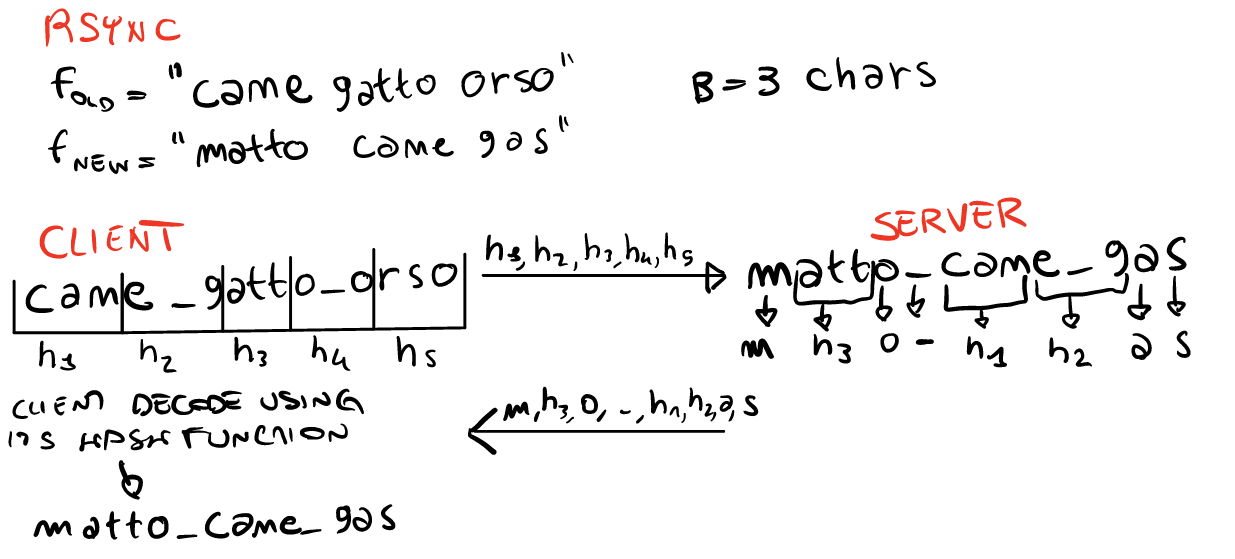
\includegraphics[width=0.8\textwidth]{Images/rsync}
				\caption{Rsync Computation steps}
				\label{img:rsync}
			\end{figure}

	\item [zsync: ] minimze server load, where computation are done in Client, and has 
			three communication steps visible in figure \ref{img:zsync}.

			\begin{figure}
				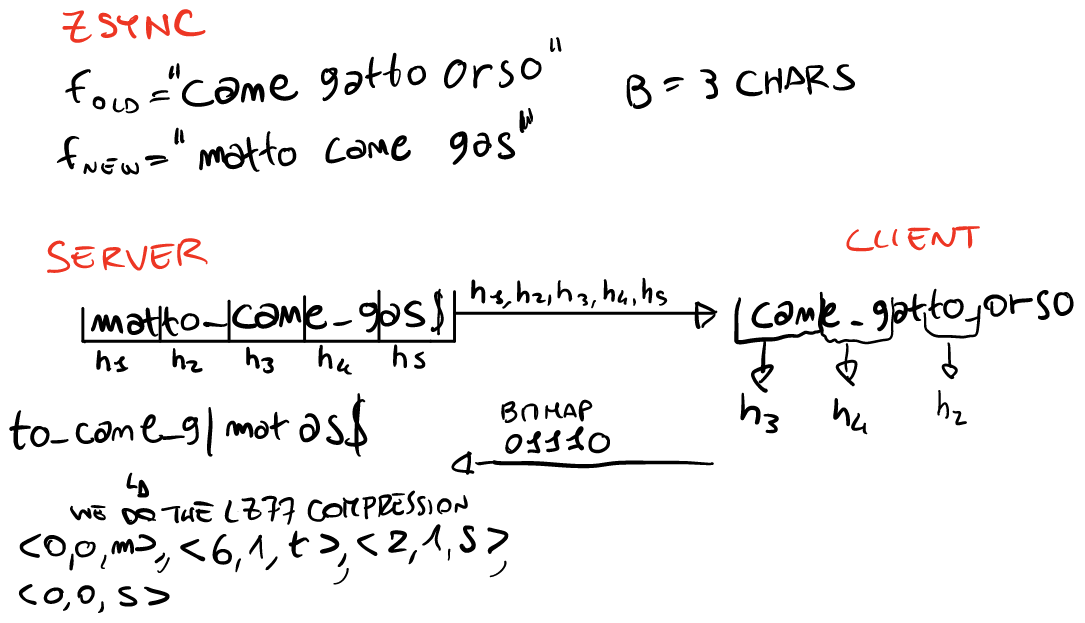
\includegraphics[width=0.8\textwidth]{Images/zsync}
				\caption{Zsync Computation steps}
				\label{img:zsync}
			\end{figure}
			The hashes of the blocks can be precalculated and stored in .zsync file
			and Server should be not overloaded, so it is better suited to 
			distribute multiple-files through network, given one .zsync.

			In our example we have a bitmap of $5$ bits because of \#blocks in
			f\_new are only five.

\end{description}

      \chapter{Document Preprocessing}
In previous chapters we have analyzed how to construct query, how to compress result,
now we will explain how to process document that has to be indexed.

Given documents to parse them we have to discover format, language and character set
used and each of them is a classification problem, but usually we use some heuristics.

After we have parsed document we tokenize them and we have the following definitions:
\begin{defi}
     Token is an istance of a sequence of characters
\end{defi}
Each such token is now a candidate for an index entry, after further processing,
that we will now present.

Sometimes there are some issues like "San Francisco" should be $1$ or $2$ tokens, or
also how to deal with hypens, apostrophe and usually this is done based with word
and is language dependent.

Another preprocessing step is to remove \emph{Stop words}, most common words in
document, and the intuition behind is that they have little semantic content
(the, a, and, to, be) and there are a lot of them ($\sim 30\%$ of postings 
for top $30$ words.\newline
Nowadays good compression techniques has reduced the space necessary to include also
stopwords and with good query optimations it is required only a small more time also
to consider it, so usually the stop words are not deleted.

We need also to “normalize” terms in indexed text and query words into the same form
so we want to match U.S.A. and USA, so we most commonly implicitly define 
\emph{equivalence classes} of terms; another preprocessing is to reduce all letters
to lower case (there is an exception to consider upper case in midsentence but often
best to lowercase everythin, since users will use lowercase regardless
of ‘correct’ capitalization).

\emph{Thesauri} is how to handle synonyms and homonyms and there are two ways to consider it: by hand-constructed equivalence classes we can rewrite to form 
equivalence-class terms and when the document contains automobile, index it 
under car-automobile (and vice-versa) or we can expand a query, so when the query
contains automobile, look under car as well.

\emph{Stemming} is the process to reduce terms to their “roots” before indexing and
suggest crude affix chopping (it is language dependent and for example 
automate(s), automatic, automation all reduced to automat).

\emph{Lemmatization} reduce inflectional/variant forms to base form (so for example
am, are,is became be)and Lemmatization implies doing “proper” reduction to 
dictionary headword form.

Many of the above features embody transformations that are language-specific and
often, application-specific and these are “plug-in” addenda to indexing.

\section{Statistical Properties of Text}
Tokens are not distributed uniformly, they follow the so called \emph{Zipf Law},
so few tokens are very frequent, a middle sized set has medium frequency and 
many are rare; the first $100$ tokens sum up to $50\%$ of the text,
and many of them are stopwords.

$k$-th most frequent token has frequency $f(k)$ approximately $1/k$, equivalently,
the product of the frequency $f(k)$ of a token and its rank $k$ is a constant
\[ k * f(k) = c \]
The number of distinct tokens grows, following with the so called \emph{Heaps Law}
\[ T = kn^b\]
where $b$ is typically $0.5$ and $n$ is the total number of tokens.\newline
The average token length grows as $\Theta(\log n)$ and interesting words 
are the ones with medium frequency (Luhn).

\section{Keyword extraction}
To extract keyword that should be consider as a single token we have several approaches that we can consider:
\begin{enumerate}
    \item Use frequency and POS (Part of Speech) tagging to obtain keywords, 
	  as can be viewed in figure \ref{img:posFrequency}.

	  \begin{figure}
		  \caption{Frequency and POS tagging approach}
		  \label{img:posFrequency}
		  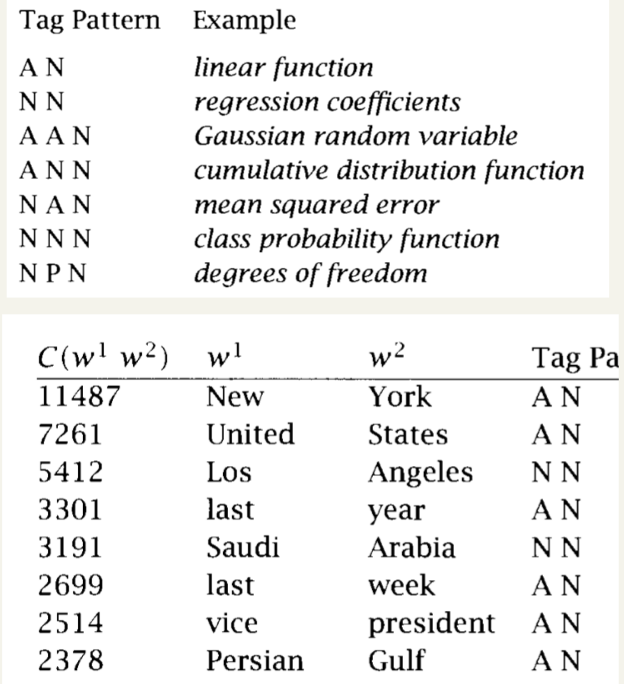
\includegraphics[width=\textwidth]{Images/posFrequency}
	  \end{figure}

    \item Often the words are not adjacent to each other and to find keyword we 
	  compute the mean and the variance of the distance, 
	  by restricting within a window, as it is possible to note in figure
	  \ref{img:meanDistance} and \ref{img:exampleDistance}.
	  If $s$ is large, the collocation is not interesting, instead if
	  $d > 0$ and $s$ very small we have interesting new keyword.

	  \begin{figure}
		\caption{Mean and Variance between Strong and some words}
		\label{img:meanDistance}
		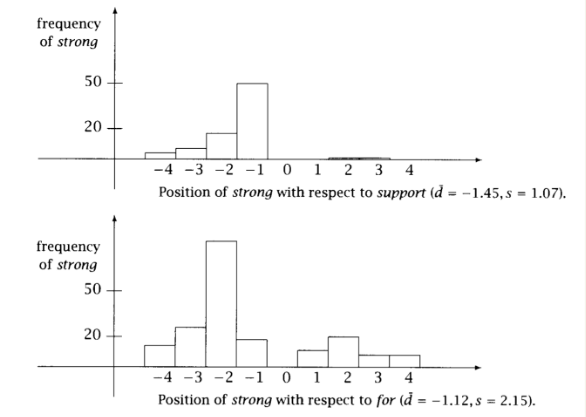
\includegraphics[width=\textwidth]{Images/meanDistance}
	  \end{figure}

	  \begin{figure}
		\caption{Example of Mean and Variance distance}
		\label{img:exampleDistance}
		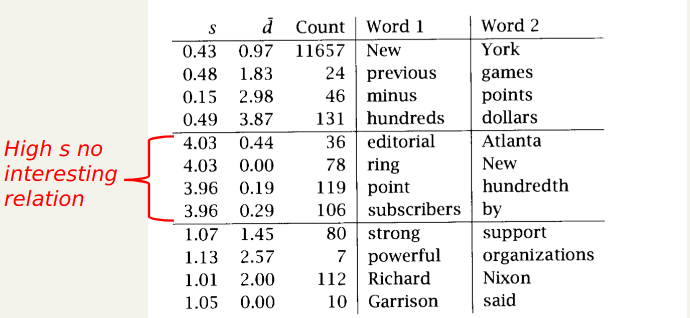
\includegraphics[width=\textwidth]{Images/exampleMeanDistance}
	  \end{figure}
    \item Pearson Chi-Square test statistics that follow a chi-squared distribution
	  arise from an assumption of independent normally distributed data,
	  which is valid in many cases due to the central limit theorem and 
	  we use $p$-value to reject the null hypothesis.

    \item \emph{RAKE} (Rapid Automatic Keyword Extraction) works on single 
	  (not much long) documents and is easily applicable to new domains, fast
	  and unsupervised.\newline
	  The Key observation of this approach is that keywords frequently contain
	  multiple words but rarely contain punctuation or stop words.

	  The input parameters are the following:
	  \begin{itemize}
		\item a set of word delimiters
		\item a set of phrase delimiters
		\item a list of stop words (or stoplist).
	   \end{itemize}
	   The RAKE approach has the following 4 step:
	   \begin{description}
		\item [Step $\#1$: ] document is split into an array of words by the specified word delimiters and 
		      this array is split into sequences of contiguous words at phrase delimiters and then stop word.

		      Words within a sequence are considered a candidate keyword, as we can see in figure 
		      \ref{img:rake}.

		      \begin{figure}
			      \caption{Extraction of Candidate keywords using RAKE}
			      \label{img:rake}
			      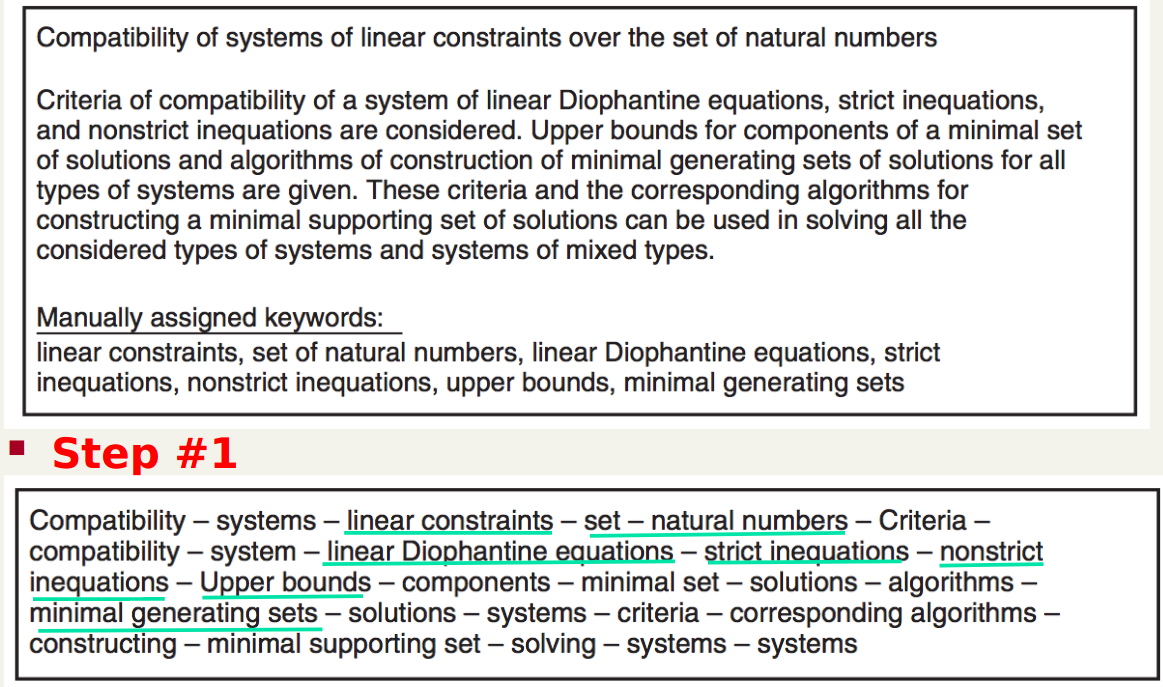
\includegraphics[width=\textwidth]{Images/rake}
		      \end{figure}

		\item [Step \#2: ] compute the table of co-occurrences and we use few metrics:
			          $freq(w)$ = total frequency on diagonal and $deg(w)$ sum over row.\newline
                                  Final score is the sum of $deg(w)/freq(w)$ for the constituting words $w$ 
				  of a keyword and in figure \ref{img:scoringCandidate} is possible to know how
				  to compute the scoring Candidate keywords.

			\begin{figure}
				\caption{Calculation of Scoring of Candidate keywords}
				\label{img:scoringCandidate}
				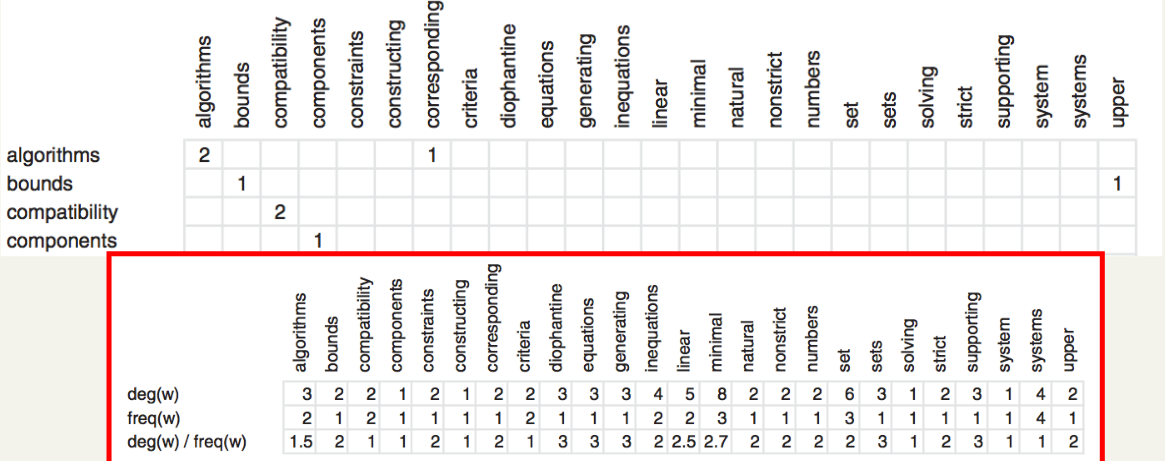
\includegraphics[width=\textwidth]{Images/rakeScoring}
			\end{figure}
		\item [Step \#3: ] identifies keywords that contain interior stop words such as axis of evil and 
			looks for pairs of keywords that adjoin one another at least twice in the same document
			and in the same order.\newline
			The score for the new keyword is the sum of its member keyword scores, as can be viewed
			in figure \ref{img:listScoring}.

			\begin{figure}
				\caption{Sorted Scoring of RAKE approach}
				\label{img:listScoring}
				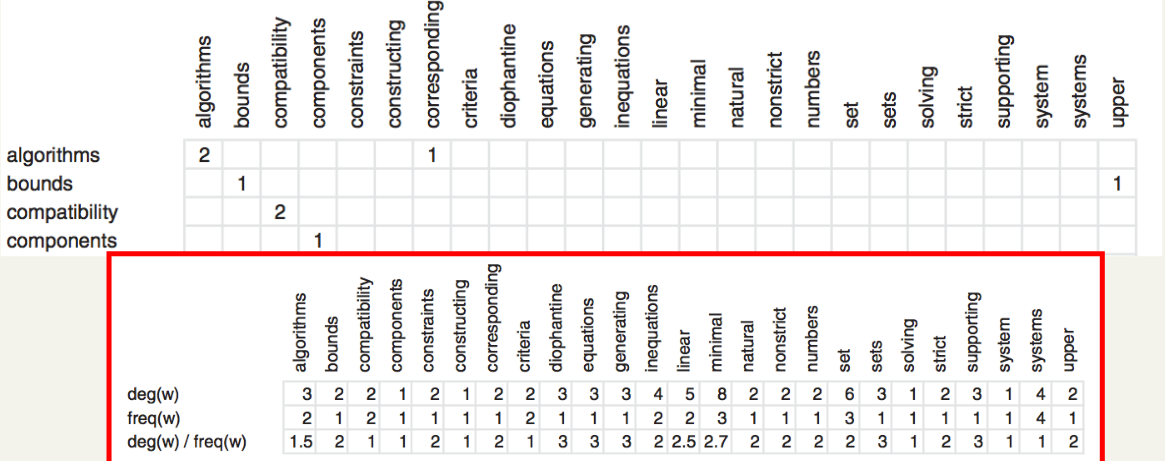
\includegraphics[width=\textwidth]{Images/rakeScoring}
			\end{figure}
		\item [Step \#4: ] we select the top one-third of sorted list of scoring obtained in previous steps
			and in figure \ref{img:rakeScoring} is possible to compare results obtained by RAKE and 
			by manual keyword extraction.

			\begin{figure}
				\label{img:rakeScoring}
				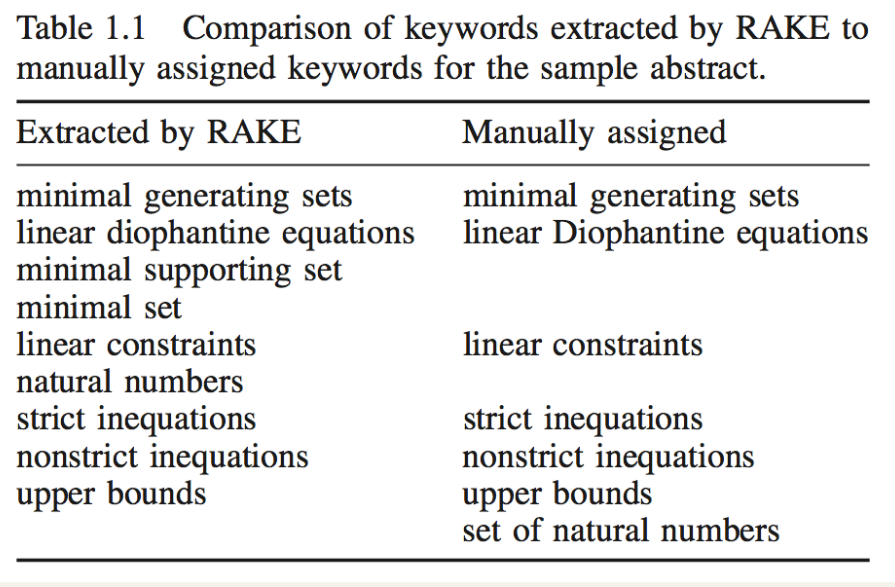
\includegraphics[width=\textwidth]{Images/rakeComparison}
			\end{figure}

	   \end{description}
\end{enumerate}


      \chapter{Data Structures for Inverted Index}
In this chapter we will analyze which data structures are used for Inverted Index and a naive approach 
consist in save in a dictionary but this cause a waste in memory and not helps in retrieve elements quickly.

To improve exact and prefix search are usually used the following data structures:
\begin{itemize}
	\item Hashing
	\item Tree
	\item Trie, also called \emph{prefix tree}, is an ordered tree data structure used to store a dynamic set
	      or associative array where the keys are usually strings.\newline
	      All the descendants of a node have a common prefix of the string associated with that node,
	      and the root is associated with the empty string; keys tend to be associated with leaves,
	      though some inner nodes may correspond to keys of interest and hence, keys are not necessarily
	      associated with every node.

	      Solves the prefix problem, but has $O(p)$ time, with many cache misses and from $10$ to $60$ (or, even more) bytes per node.

\end{itemize}
To improve our search we exploits $2$-level caching indexing, that improve search, typically $1$ I/O $+$ in-mem comparison and 
improve also space requirement, because we use a trie built over a subset of string and front-coding over buckets.\newline
A disadvantage is the trade-off between speed and space, caused by bucket size.

Front-coding is a type of delta encoding compression algorithm whereby common prefixes or suffixes and their lengths 
are recorded so that they need not be duplicated and this algorithm is particularly well-suited for compressing sorted data,
as we can see in figure \ref{img:front-coding}.

\begin{figure}
	\caption{Example of Front Coding}
	\label{img:front-coding}
	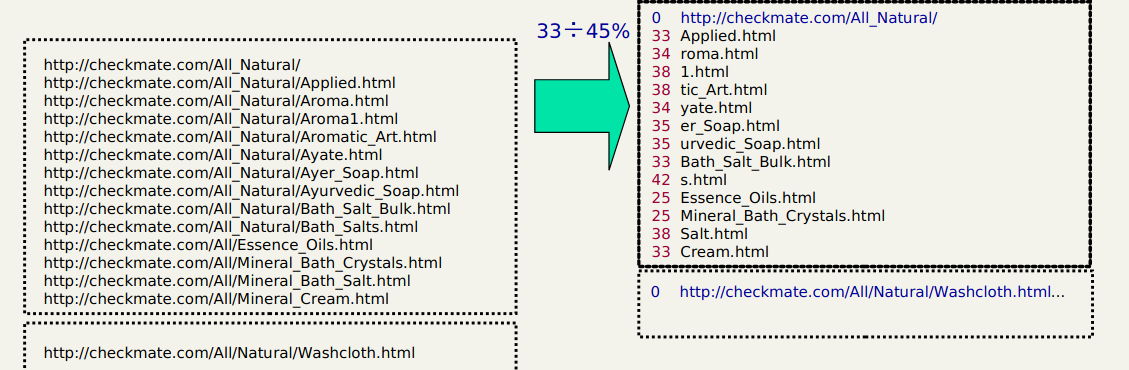
\includegraphics[width=\textwidth]{Images/frontCoding}
\end{figure}

\section{Correction Queries}
Spell correction has $2$ principal uses:
\begin{enumerate}
    \item Correcting document(s) to be indexed.
    \item Correcting queries to retrieve “right” answers.
\end{enumerate}
There are two approaches that can be used:
\begin{enumerate}
    \item Isolated word: check each word on its own for misspelling.
    \item Context-sensitive is more effective and look at surrounding words.
\end{enumerate}
To correct isolated word there is a lexicon from which the correct spellings come and two basic choices for this are
a standard lexicon such as Webster’s English Dictionary or an “industry-specific” lexicon, that is specific for a field and where
we can use mining algorithms to derive possible corrections.

Isolated word correction consist that given a lexicon and a character sequence $Q$, return the words in the lexicon closest
to $Q$; for estabilish what's closest we will study several measures (we will study Edit distance, Weighted edit distance and
$n$-gram overlap).

Edit Distance is generally found by dynamic programming and consist given two strings $S1$ and $S2$, to find the minimum number of 
operations to convert one to the other (Operations are typically character-level insert, delete, replace, with possibility of also transposition.

In figure \ref{img:editDistance} is possible to find how is computed the edit distance and we compute the table of distance from 
bottom to top, using equation described in the figure.

\begin{figure}
	\caption{Equation for computing Edit Distance}
	\label{img:editDistance}
	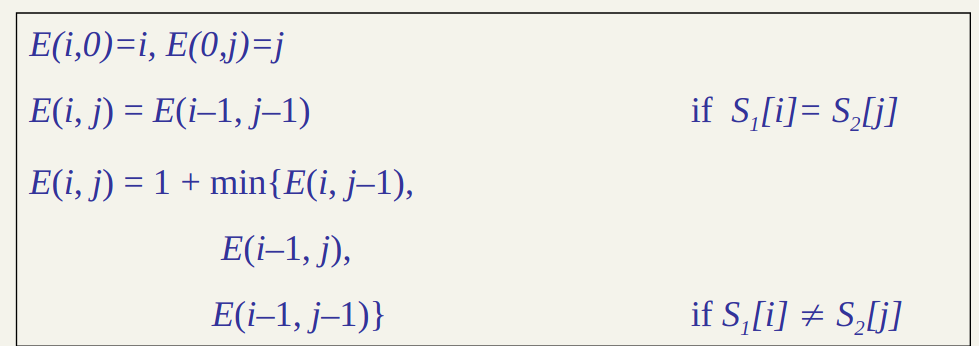
\includegraphics[width=\textwidth]{Images/editDistance}
\end{figure}
We introduce now \emph{Weighted edit distance}, where the weight of an operation depends on the character(s) involved and 
meant to capture keyboard errors, as for example $m$ is more likely to be mis-typed as $n$ than as $q$.\newline
Therefore, replacing $m$ by $n$ is a smaller cost than by $q$ and requires weighted matrix as input.

We create two dictionaries $D_1 = \{ strings \}$ and $D_2 = \{ strings of D1 with one deletion \}$; for a query we have to 
do 1 search in $D_1$ in perfect match, $1$ query in $D_2$ to find $1$-char less, $p$ queries to find $P$ with $1$-char less from $D_2$ to $D_1$
and in the end $p$ queries to find substitution in $D_2$ from $P$ with $1$-char less.

We need $2p + 2$ hash computations for $P$ and the positive aspects are that is CPU efficient, no cache misses for computing P’s hashes,
but $O(p)$ cache misses to search in $D_1$ and $D_2$, instead negative aspects are large space because of the many strings in $D_2$ 
which must be stored to search in the hash table of D2, unless we avoid collision and the presence of false matches.

A better approach consist to use overlap distance, where we use the $k$-gram index contains for every $k$-gram all terms including
that $k$-gram and we append $k-1$ symbol \$ at the front of each string, in order to generate a number $L$ of $k$-grams 
for a string of length $L$

We select terms by threshold on matching $k$-grams and if the term is $L$ chars long (it consists of $L k$-grams) and if $E$
is the number of allowed errors ($E*k$ of the $k$-grams of $Q$ might be different from term’s ones because of the $E$ errors) and 
so at least $L – E*k$ of the $k$-grams in $Q$ must match a dictionary term to be a candidate answer and if ED is required,
post-filter results with dynamic programming.

We enumerate multiple alternatives and then need to figure out which to present to the user for “Did you mean?" and we use heuristics:
the alternative hitting most docs and query log analysis + tweaking (done for especially popular, topical queries), anyway
spell-correction is computationally expensive and is run only on queries that matched few docs.

We introduce now how to deal with \emph{wildcard queries} and to deal we use \emph{permuterm index}, where we have the 
following possible queries:
\begin{itemize}
    \item X lookup on X\$
    \item X* lookup on   \$X*
    \item *X lookup on X\$*
    \item *X* lookup on X*
    \item X*Y lookup on Y\$X*
\end{itemize}
The permuterm query processing consist to rotate query wild-card to the right so P*Q become Q\$P* so now we 
use prefix-search data structure and a problem of Permuterm is that has $\approx 4x$ lexicon size (an empirical observation for English).

\emph{Soundex} is a class of heuristics to expand a query into phonetic equivalents, it is language specific used mainly for names
and was invented for the U.S. census in 1918.\newline
We introduce now the original algorithm that consist to turn every token to be indexed into a reduced form consisting of $4$ chars
and do the same with query terms, so we build and search an index on the reduced forms (in figure \ref{img:soundex} are indicated
all steps of basic algorithm).

\begin{figure}
	\caption{Soundex basic Algorithm}
	\label{img:soundex}
	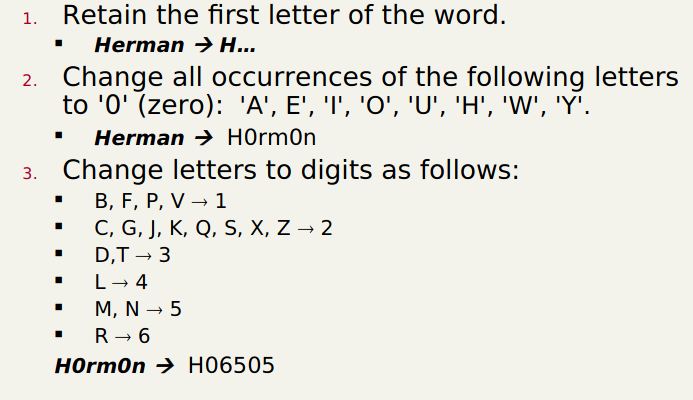
\includegraphics[width=\textwidth]{Images/soundex1}
	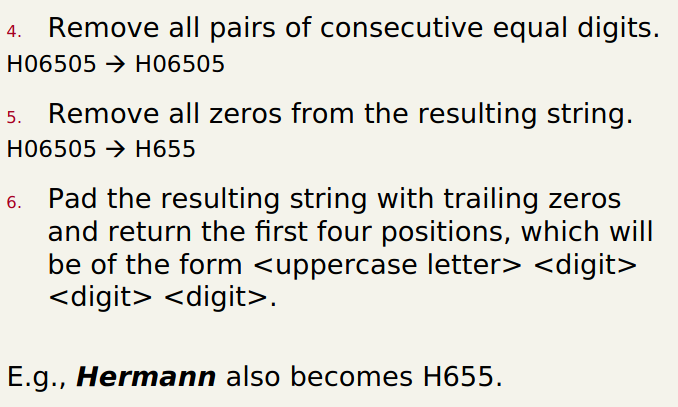
\includegraphics[width=\textwidth]{Images/soundex2}
\end{figure}
Soundex is the classic algorithm, provided by most databases (Oracle, Microsoft, and so on) but is not very useful for information retrieval;
is okay for “high recall” tasks (e.g., Interpol), though biased to names of certain nationalities, so other algorithms
for phonetic matching perform much better in the context of IR.



      \chapter{Query Processing}
In this chapter we will introduce how to answer queries such as “stanford university” as a phrase and 
thus the sentence “I went at Stanford my university” is not a match.

The first approach consist to use the \emph{$2$-word indexes}, so for example the text "Friends, Romans, Countrymen" would generate the biwords
friends romans and romans countrymen, so each of these $2-$words is now an entry in the dictionary and the two-word phrase query-processing is immediate.

Longer phrases are processed by reducing them to bi-word queries in AND, so "stanford university palo alto"
can be broken into the Boolean query on biwords, such as "stanford university AND university palo AND palo alto".\newline
The problem of this approach is that need the docs to verify, can have false positives and index blows up, so a better approach consist to \emph{positional indexes},
where in the postings we store for each term and  document the position(s) in which occurs; typically queries happens with free text,
so just a set of terms typed into the query box common on the web and users prefer docs in which query terms
occur within close proximity of each other so we would like scoring function to take this into account.

With positional index size we can compress position values/offsets and nevertheless, a positional index expands
postings storage by a factor $2$-$4$ in English, it is now commonly used because of the power and usefulness of phrase and proximity queries, 
and we introduce now the \emph{Soft-AND}, used to solve phrase query, which algorithm is visible in figure \ref{img:softAnd}.

\begin{figure}
	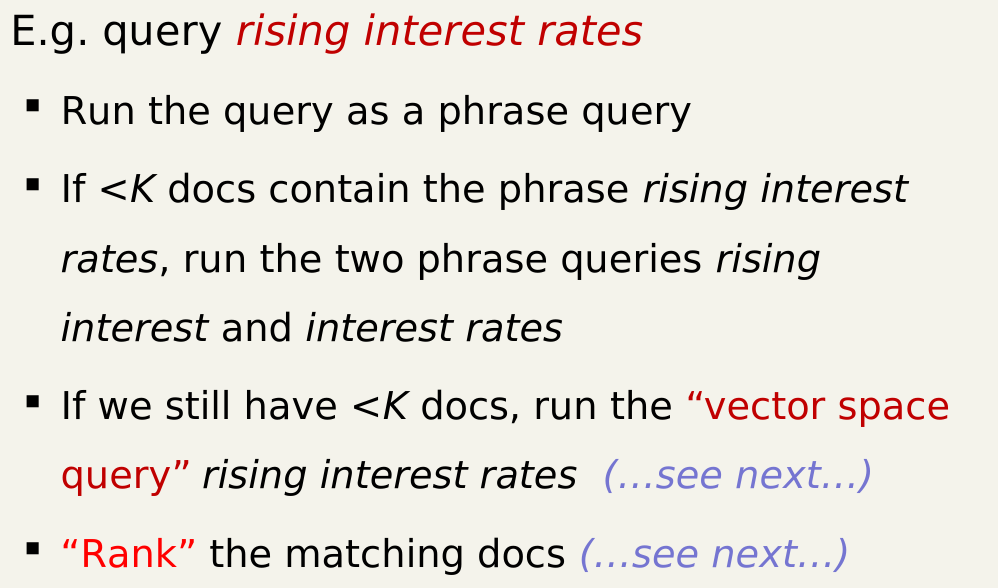
\includegraphics[width=\textwidth]{Images/softAnd}
	\caption{SoftAnd Algorithm procedure}
	\label{img:softAnd}
\end{figure}
To achieve better results we cache and there are two opposite approaches:
\begin{enumerate}
	\item Cache the query results and exploits query locality.
	\item Cache pages of posting lists and so exploits term locality.
\end{enumerate}
In figure \ref{img:cacheQuery} is possible to note how consist the cache for query and/or postings.

\begin{figure}
	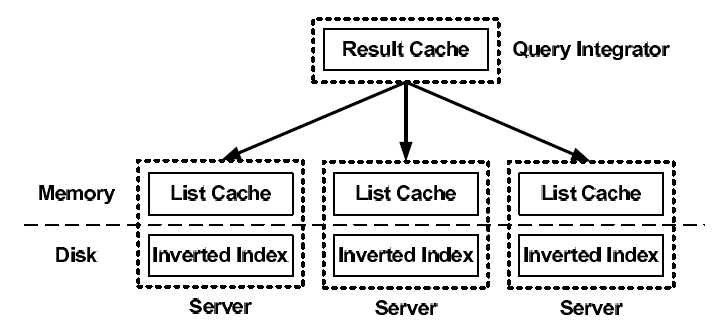
\includegraphics[width=\textwidth]{Images/cacheQuery}
	\caption{Composition of Cache on Query/Postings}
	\label{img:cacheQuery}
\end{figure}
To have faster query we can use \emph{tiered query}, where we break postings up into a hierarchy of lists, so inverted index thus broken up into tiers of
decreasing importance and at query time we use top tier unless it fails to yield $K$ docs and if so drop to lower tiers, as we can note in figure \ref{img:tiered}.

\begin{figure}
		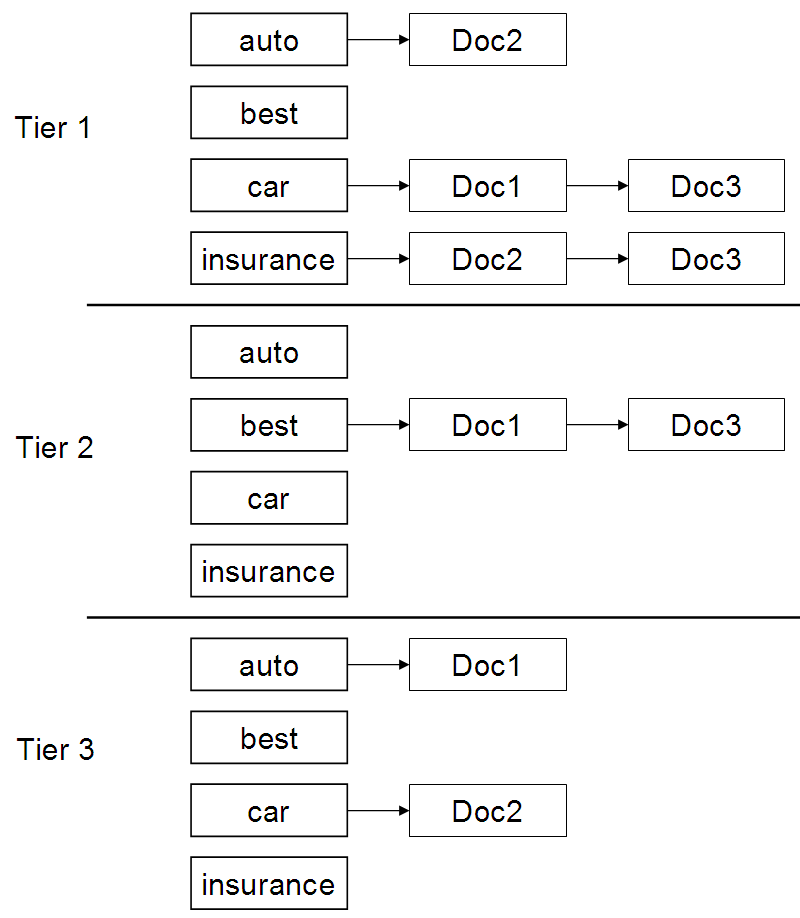
\includegraphics[width=0.7\textwidth]{Images/tieredIndex}
	\caption{Example of Tiered Queries}
	\label{img:tiered}
\end{figure}



      \chapter{Document ranking}
We consider document as binary vector $X, Y \in \{0, 1\}^D$ and we start to use 
as score the \emph{overlap measure} defined as 
\[ |X \cap Y| \]
and in figure \ref{img:overlap} is possible to note that it provides a measure without information.

\begin{figure}
	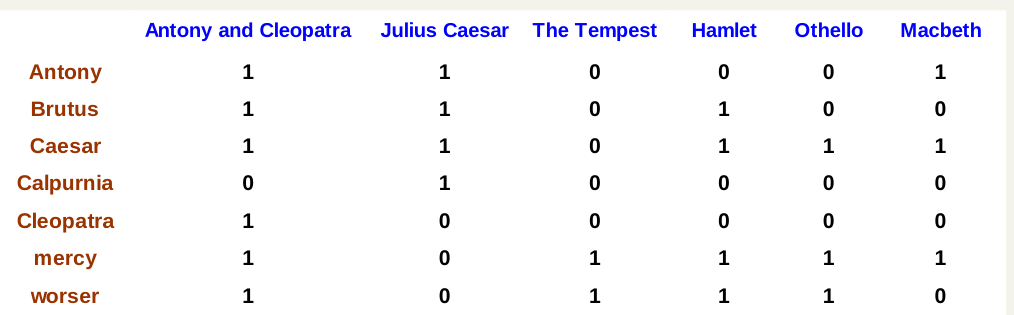
\includegraphics[width=0.8\textwidth]{Images/exampleOverlap}
	\caption{Example of Overlap measure}
	\label{img:overlap}
\end{figure}
Better measures are the following:
\begin{description}
	\item [Dice coefficient: ] with respect to average of $\#$ terms, is not respect triangular rules and it is defined as 
		\[ 2 |X \cap Y| / (|X| + |Y|) \]
	\item [Jaccard coefficient: ] with respect to possible terms, it respects the triangular rules, and it is defined as 
		\[ |X \cap Y| / |X \cup Y| \]
\end{description}
Overlap matching doesn’t consider term \emph{frequency} in a document, term \emph{scarsity} in collection and length of documents so 
score should be normalized, and to do that we introduce now a famous weight \emph{tf-idf}, defined as
\[ w_{t, d} = tf_{t, d} \log \frac{n}{n_t} \]
where we have $tf_{t, d}$ defined as number of occurences of term $t$ in document $d$ and $idf_t = \log (n/n_t)$, 
where $n$ is the number of documents and $n_t$ is the number of docs containing term $t$.

We have also that the distance is a bad idea, as it is possible to note in figure \ref{img:exDistance}, and we define
now the \emph{cosine} measures as follows
\begin{figure}
	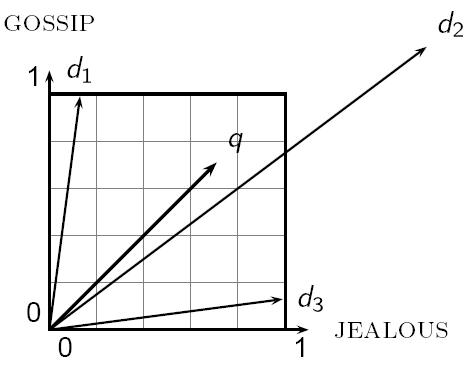
\includegraphics[width=0.7\textwidth]{Images/distanceProblem}
	\caption{Example of problem in distance}
	\label{img:exDistance}
\end{figure}
\[ \cos \alpha = \frac{v * w}{\norm{v} * \norm{w}} \]
The problem is this approach is that it is easy to spam and also that it is computationally infeasible,
cause we have to compute the dot-product $v * w$.

We define also \emph{cosing} measure between query and document in the following way
\[ \cos(q, d) = \frac{q * d}{\norm{q} \norm{d}} = \frac{\sum _{i=1}^{|D|} q_i * d_i}{\sqrt{\sum_{i=1}^{|D|} q_i^2} * \sqrt{\sum _{i=1}^{|D|} d_i^2}} \]
where $q_i$ is the tf-idf weight of term $i$ in the query and $d_i$ is the tf-idf weight of term $i$ in the document.

To help to compute the cosine between query and document we use inverted lists and also that
\[ w_{t, d} = tf_{t, d} \log (n / n_t) \]
that can be computed simultaneously since for every term $t$, we have in memory the length $n_t$ of its posting list and for 
every docID $d$ in the posting list of term $t$, we store its frequency $tf_{t, d}$ which is typically small and 
thus stored with unary/gamma.

In figure \ref{img:computeCosine} it possible to note the algorithm to compute the cosine score and also that 
vector space is okay for bag-of-words queries, that provides clean metaphor for similar-document queries and 
it is not a good combination with operators: boolean, wild-card, positional, proximity.

It was used in first generation of search engines, invented before "spamming" web search, since 
inject webpage with spamming elements that will confuse search engines.

\begin{figure}
	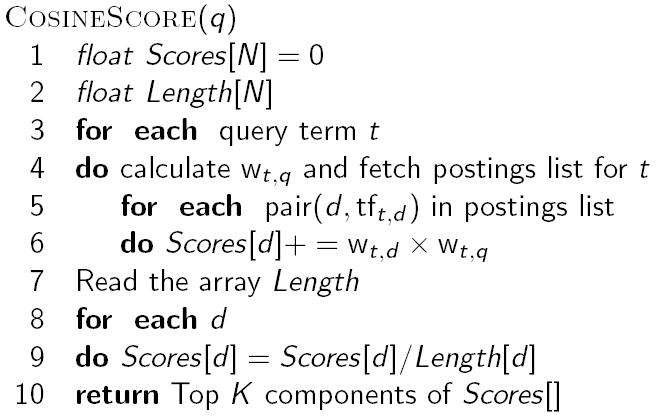
\includegraphics[width=0.8\textwidth]{Images/computeCosineScore}
	\caption{Algorithm to compute the cosine score}
	\label{img:computeCosine}
\end{figure}

\section{Top-k documents}
The computation of $\cos$ is very costly, so to compute the top$-k$ 
documents we find a set $A$ of contenders, with $k < |A| << N$,
where set $A$ does not necessarily contain all top$-k$, but has many
documents from among the top$-k$ and return the top$-k$ docs in $A$,
according to the score; the same approach is also used for other 
scoring functions and we will look at several schemes following this approach.

To select the $A$ docs we consider docs containing at least one query term
and we use the following approaches:
\begin{itemize}
    \item for multi-term queries, compute score for docs containing
	  most query terms (say at least $q-1$ out of $q$ terms of the 
	  query and imposes a "soft AND" on queries seen on web search engines.

   \item Use only high-idf query terms, where high-IDf means short posting
	 lists (rare terms) so we only accumulate ranking for documents 
	 in those posting lists, with an approach visible
	 in figure \ref{img:highIDF}.

	 \begin{figure}
		 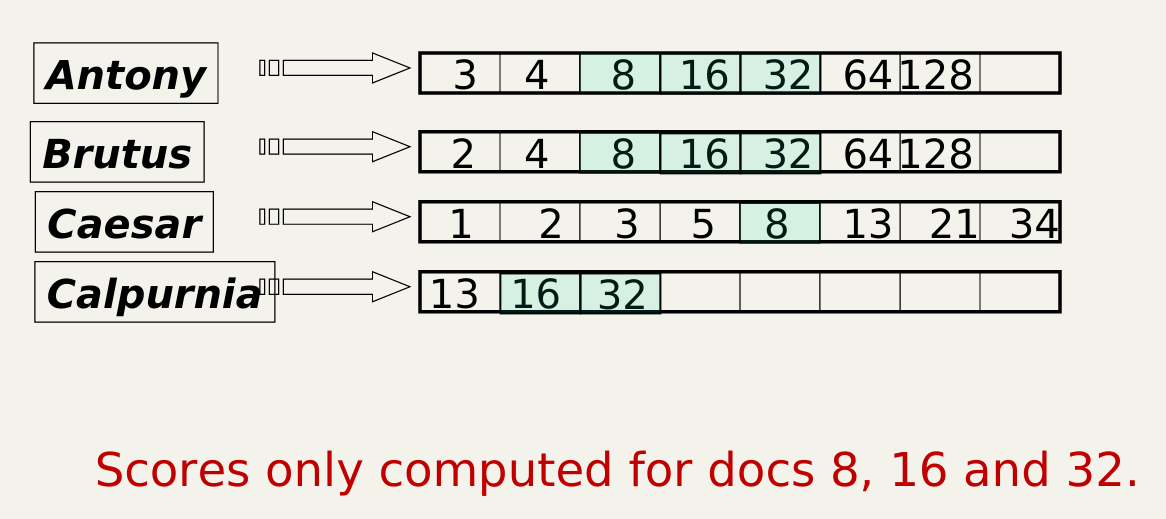
\includegraphics[width=0.8\textwidth]{Images/highIDF}
		 \caption{Top-k documents using high-IDF}
		 \label{img:highIDF}
	 \end{figure}

   \item We use \emph{Champion lists}, where we assign to each term, its
	 $m$ best documents, so if $|Q| = q$ terms we merge their preffered
         lists ($\leq mq$ answers) and we compute the cosine between $q$
	 and these docs, and choose the top.\newline
	 This approach need to pick $m > k$ to work well empirically.

   \item We use \emph{Fancy-hits} heuristic, where we assign docID by
	 decreasing PR weight, sort by docID $=$ order by decreasing 
	 PR weight, so we define $FH(t) = m$ docs for $t$ with 
	 highest $tf$-$idf$ weight and we define $IL(t)$ as the rest.

	 To search a $t-$term query we use a double approach:
	 \begin{enumerate}
	    \item consider $FH$ and we compute the score of all docs in their
		  $FH$, like champion lists and keep the top$-k$ docs.
	    \item consider then $IL$, so we scan $IL$s and check the common 
		  docs: compute the score, possibly insert them into 
		  the top$-k$ and stop when $m$ docs have been checked or
		  the $PR$ score becomes smaller than some threshold.
	 \end{enumerate}
         In figure \ref{img:fancy} it is possible to understand when we 
	 stop to consider elements in fancy-hits approach.

	 \begin{figure}
		 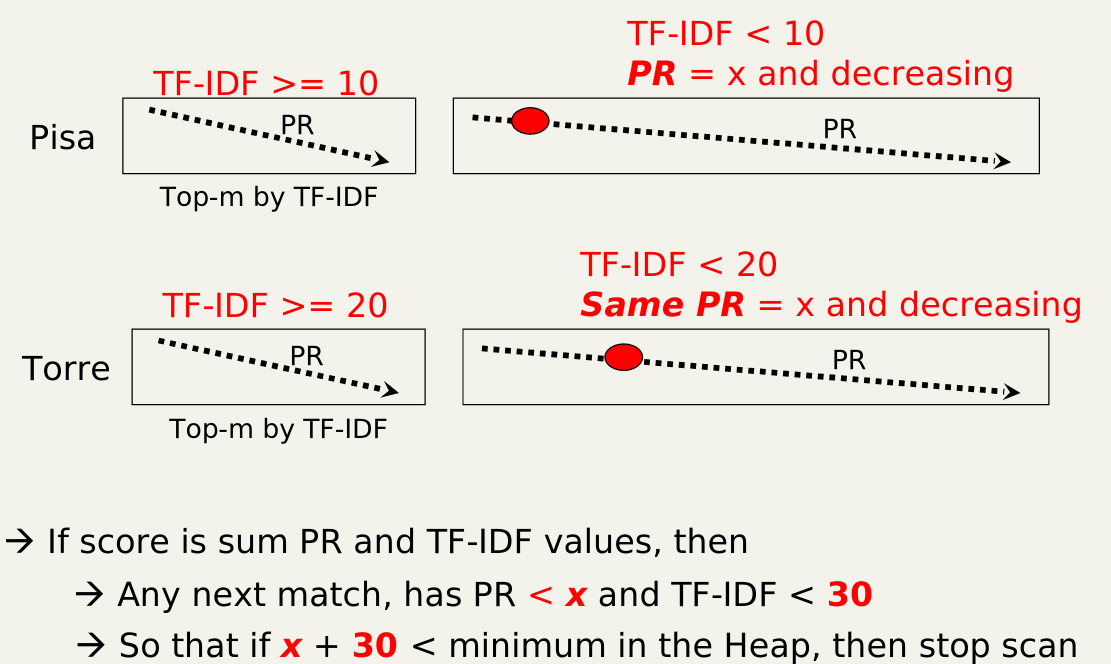
\includegraphics[width=0.8\textwidth]{Images/fancyHits}
		 \caption{Stop criteria for Fancy-hits approach}
		 \label{img:fancy}
	 \end{figure}
	 We assign to each document a query-independent quality score in
	 $[0, 1]$ to each document $d$ (denote this by $g(d)$ and thus
	 a quantity like the number of citation is scaled into $[0, 1]$.\newline
	 We can combine champion lists with $g(d)$ ordering, or maintain
	 for each term a champion list of the $r > k$ docs with highest 
	 $g(d) + tf-idf_{td}$; $g(d)$ may be the PageRank and seek top $k$
	 results from only the docs in these champion lists.

    \item The last but not least approach consist to clustering, where we 
	  pick $\sqrt N$ docs at random (call these leader) and for every
	  other doc we precompute nearest leader, so docs are attached
	  to a leader and each leader has $\sim N$ followers.

	  It process a query as follows:
	  \begin{enumerate}
	      \item Given query $Q$ find its nearest leader $L$.
	      \item Seek $K$ nearest docs from among $L$'s followers.
	  \end{enumerate}
	  We use a random sampling because it is fast and leaders 
	  reflect data distribution, anyway we will study now a general 
	  variant, which consist that each followe is attached to the 
	  nearest leader, but given now the query find for example $b=4$
	  nearest leaders and their followers.\newline
	  For them compute the scores and then take the top$-k$ ones
	  and that can recur on leader/follower construction.

\end{itemize}

\section{Exact top-$k$ documents}
In this section we will consider the problem that given a query $Q$
find the exact top $k$ docs for $Q$, using some ranking function $r$.

The simplest strategy consist to:
\begin{enumerate}
    \item Find all documents in the intersection.
    \item Compute score $r(d)$ for all these documents $d$.
    \item Sort results by score. 
    \item Return top $k$ results.
\end{enumerate}
The problem of this approach is that the score computation is a large fraction
of the CPU work on a queery and our goal is to cut CPU usage for scoring,
without compromising on the quality of results and the basic idea consist
to avoid scoring docs that won't make it into the top $k$.

A better approach consist to \emph{WAND} technique, a pruning method which
uses a max heap over the real document scores, and there is a proof that 
the docIDs in the heap at the end of the process are the exact top$-k$.

Basic idea of this approach come from the \emph{branch and bound}, so 
we maintain a running threshold score ($k$-th highest score computed so far),
we prune away all docs whose scores are guaranteed to be below the threshold
and in the end we compute exact scores for only the unpruned docs.

In WAND postings are ordered by docID, and we assume a special iterator on the 
postings that can go to the first docID $>$ X (using skip pointers or 
Elias-Fano's compressed lists) and this iterator moves only to the right,
to larger docIDs.

We assume also that $r(t, d)$ is the score of $t$ in $d$ and the score of the 
document $d$ is the sum of the scores of query terms; also for each query 
term $t$, there is some upper-bound $UB(t)$ such that, for all $d$
\[ r(t, d) \leq UB(t) \]
and these values are pre-computed and stored.

We keep inductively a threshold $\theta$ such that for every document $d$
within the top-$k$ it holds that $r(d) \geq \theta$; $\theta$ can be initialized
to $0$ and it is raised whenever the "worst" currently found top$-k$ has a 
score above the threshold.

In figure \ref{img:wand} it is possible to note the execution of WAND approach
and in test wand leads to a $90\%$ reduction in score computation (better
gains are on longer queries and gives us also safe ranking.

\begin{figure}
	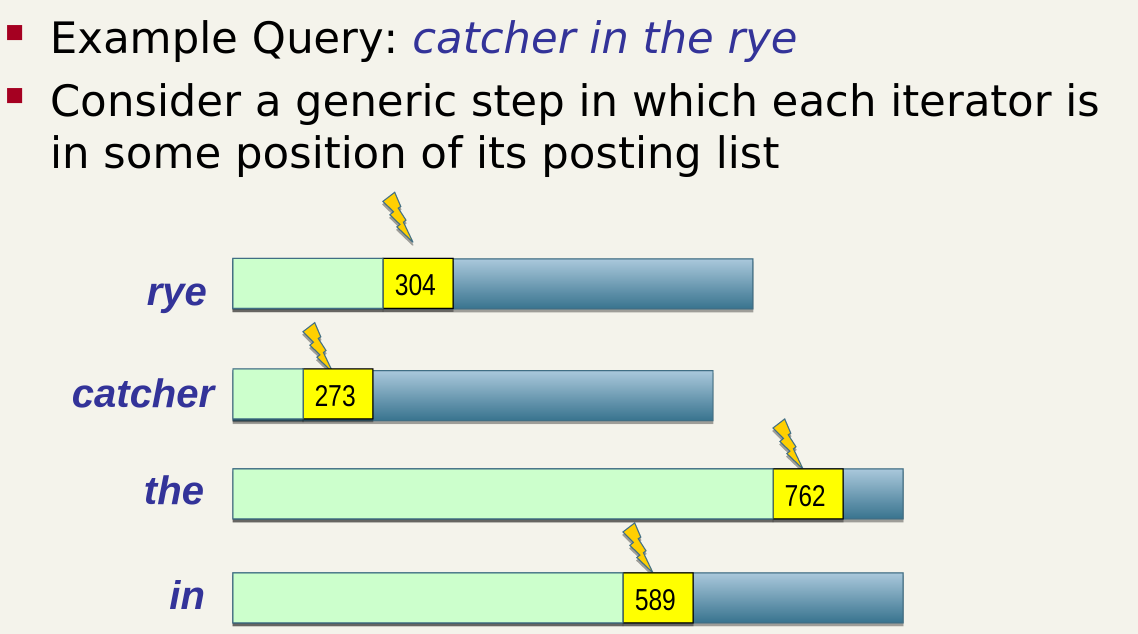
\includegraphics[width=0.4\textwidth]{Images/wand1}
	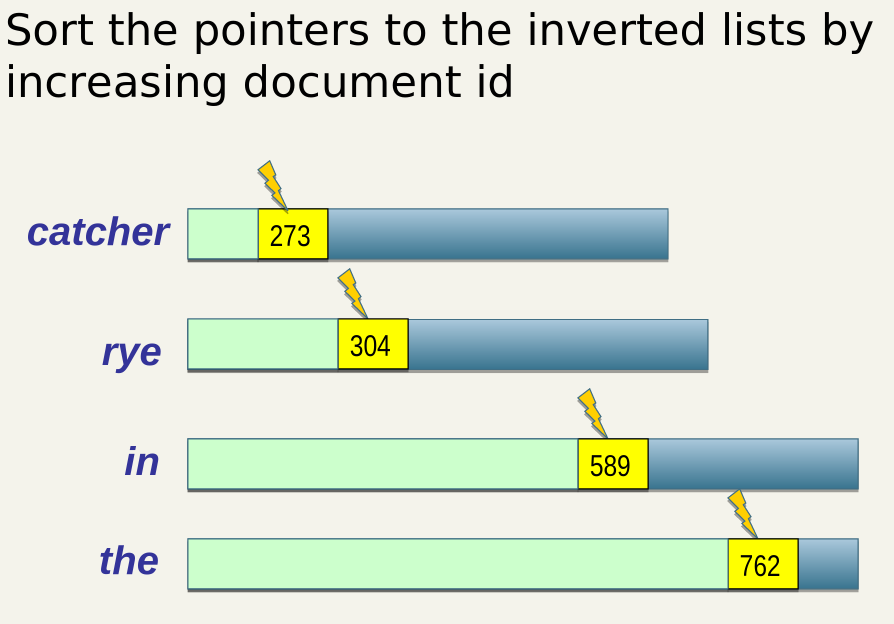
\includegraphics[width=0.4\textwidth]{Images/wand2}
	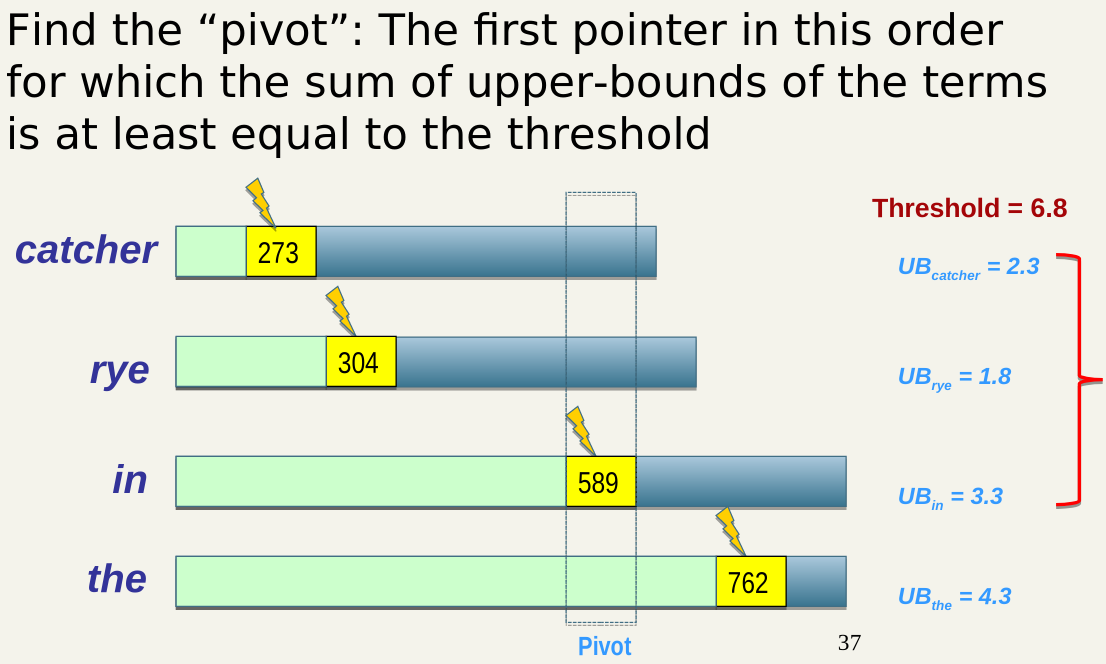
\includegraphics[width=0.4\textwidth]{Images/wand3}
	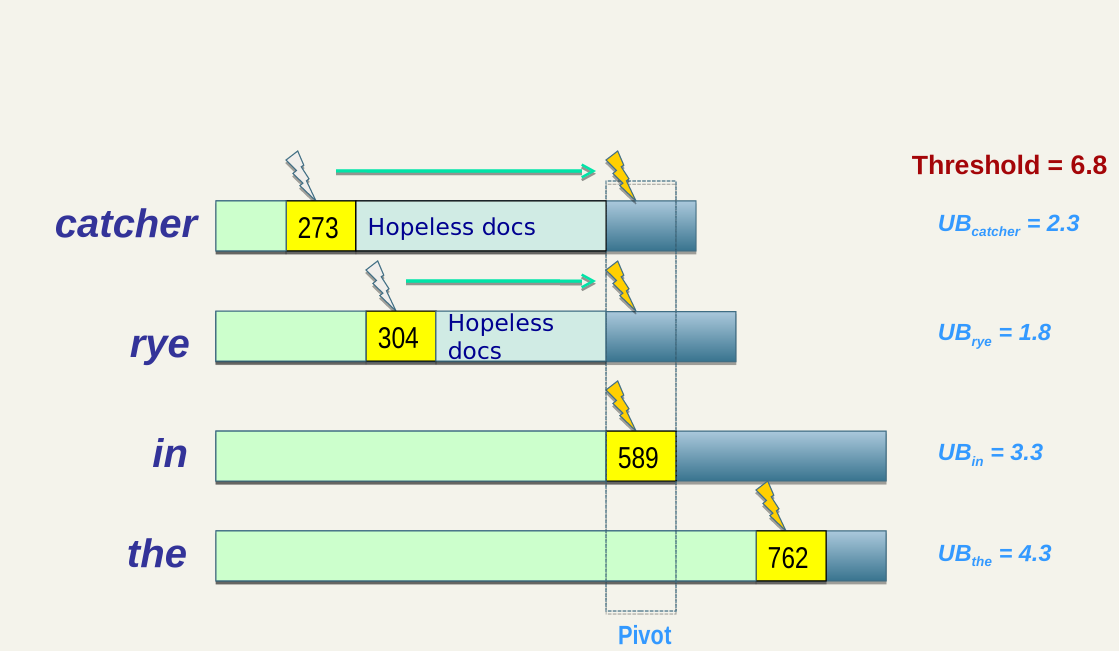
\includegraphics[width=0.4\textwidth]{Images/wand4}
	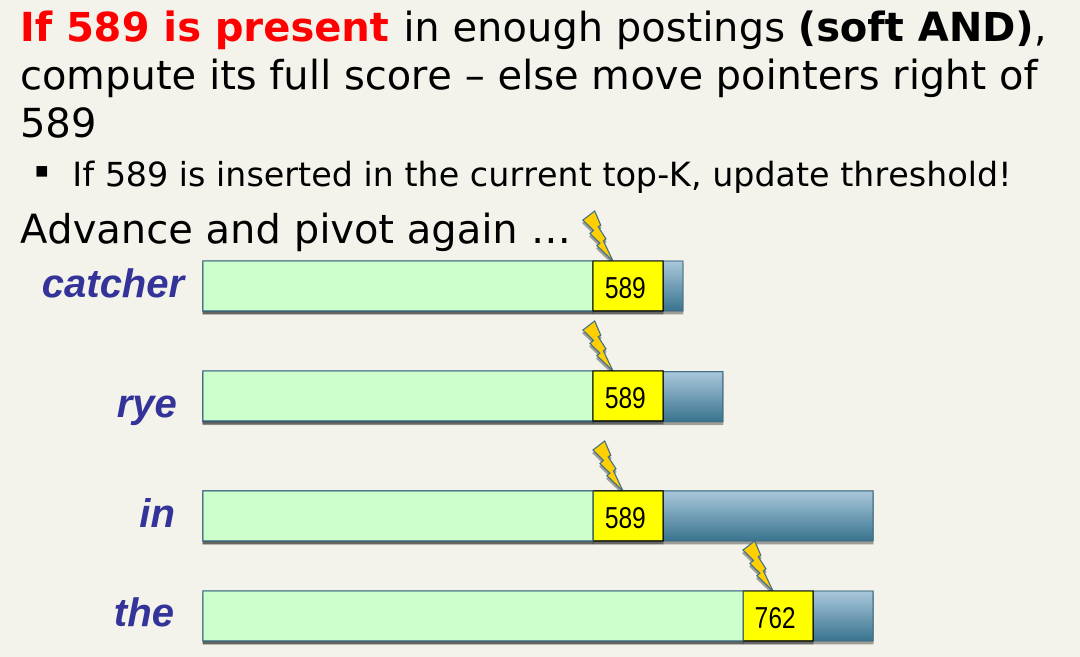
\includegraphics[width=0.4\textwidth]{Images/wand5}
	\caption{Execution of Wand algorithms steps}
	\label{img:wand}
\end{figure}

In wand $UB(t)$ was over the full list of $t$ and to improve this we add the 
following: partition the list into blocks and store for each block $b$ the 
maximum score $UB_b(t)$ among the docIDs stored into it, so we have 
the new algorithm \emph{block-max WAND}, that consist in $2-$levels check.

As in previous WAND we compute $p$, pivoting docIDs via threshold $\theta$
taken from the max-heap and let also $d$ be the pivoting docID in list($p$).

The new aspects executed in block-max variant is visible in figure 
\ref{img:blockWand}.

\begin{figure}
	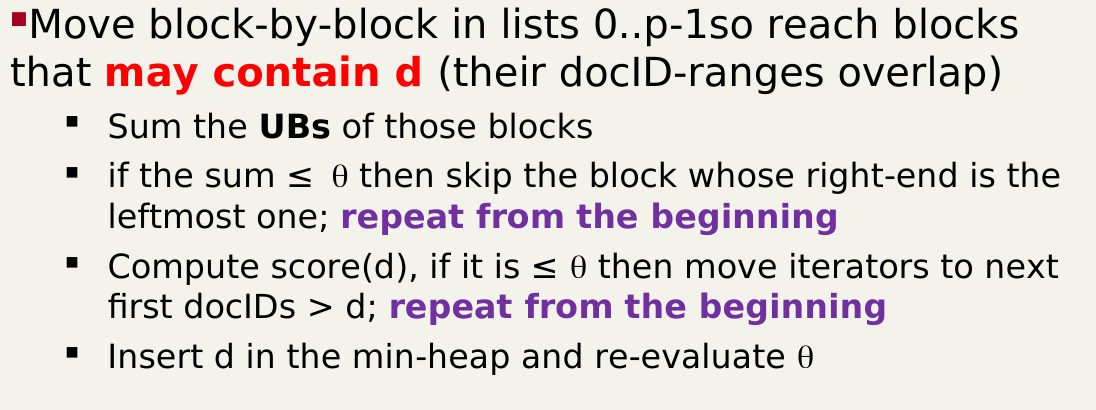
\includegraphics[width=0.7\textwidth]{Images/blockWand}
	\caption{Block-max Wand approach extension}
	\label{img:blockWand}
\end{figure}

\section{Relevance Feedback}
Relevance feedback consist that user give feedback on relevance of docs
in initial set of results, with an approach that consist on
\begin{itemize}
    \item User issues a (short, simple) query.
    \item The user marks some results as relevant or non-relevant.
    \item The system computes a better representation of the information
	  need based on feedback.
    \item Relevance feedback can go through one of more iterations.
\end{itemize}
A measure communly used is the \emph{Rocchio (SMART)} which is defined as
\[ q_m = \alpha q_0 + \beta \frac{1}{|D_r|} \sum _{d_j \in D_r} d_j -
         \gamma \frac{1}{|D_{nr}|} \sum _{d_j \in D_{nr}} d_j \]
where $D_r$ is the set of known relevant doc vectors, $D_{nr}$ is the 
set of known irrelevant doc vectors, $q_m$ is modified query vector
and $q_0$ is the original query vector.

With this formula new query moves toward relevant documents and away
from irrelevant documents, but the problem of this relevant approach 
consist that users are often reluctant to provide explicit feedback,
also it's often harder to understand why a particular document was retrieved
after applying relevance feedback and in the end there is no clear evidence
that relevance feedback is the "best use" of the user's time.

An improvement consist to \emph{Pseudo relevance feedback}, which
automates the "manual" part, so we retrieve a list of hits for the
user's query, assume that the top $k$ are relevant and do relevance feedback.

This pseudo approach works very well on average, but can go horribly wrong
for some queries and several iterations can cause query drift.

In relevance feedback, users give additional input (relevant/non-relevant)
on documents, which is used to reweight terms in the documents and 
in query expansion, users give additional input (good/bad search term)
on words or phrases; ways to augment the user query are manual thesaurus
(costly to generate using for example MedLine), global analysis (static)
done on all docs in collection using automatically derived thesaurus and 
refinements based on query-log mining and the last approach consist to
local analysis (dynamic), which consist to analysis of documents in result set.

\section{Quality of Search Engine}
In this section we will consider the quality of search engine, and provide
so measure functions to evaluate search engine but also all information
retrieval systems.

Some measures to evaluate can be how fast does it index, how fast does
it search, expressiveness of the query language and these criteria are
measurable but the key measure is the \emph{user happiness}, because
useless answers won't make a user happy, so we introduce two important 
measures: \emph{precision} and \emph{recall}.

In figure \ref{img:precisionRecall} is possible to note visually what 
mean these measure, but in words precision is the percentual
of docs retrieved that are relevant, instead recall is the 
percentual of docs relevant that are retrieved.

\begin{figure}
	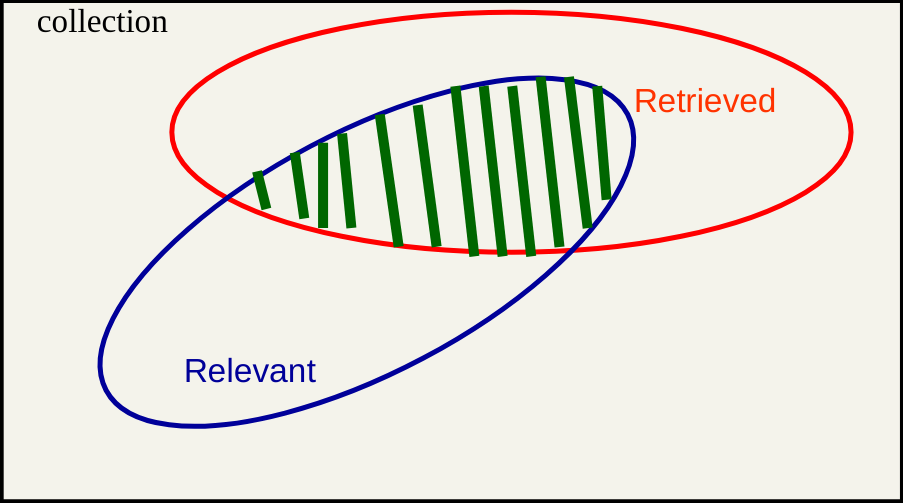
\includegraphics[width=0.8\textwidth]{Images/precisionRecall}
	\caption{Meaning of Precision and Recall}
	\label{img:precisionRecall}
\end{figure}

In figure \ref{img:relevantMatrix} is possible to note the table between
retrieved and relevant so from them can be derived the formula
of these criteria
\begin{align*}
	P & = \frac{TP}{TP + FP} \\
	R & = \frac{TP}{TP + FN} \\
\end{align*}
In the end in figure \ref{img:imagePrecision} is possible to note
the relation between precision and recall displayed by a plot.

\begin{figure}
	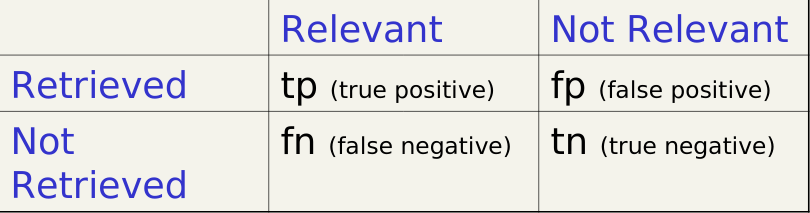
\includegraphics[width=0.8\textwidth]{Images/relevantMatrix}
	\caption{Relation between Relevant and Retrieved documents}
	\label{img:relevantMatrix}
\end{figure}
Last but not least measure used is the \emph{F measure}, that it is 
a combined measure (weighted harmonic mean) defined as 
\[ F = \frac{1}{\alpha \frac{1}{P} + (1 - \alpha) \frac{1}{R}} \]
People usually use balanced $F_1$ measure with $\alpha = 0.5$.

\begin{figure}
	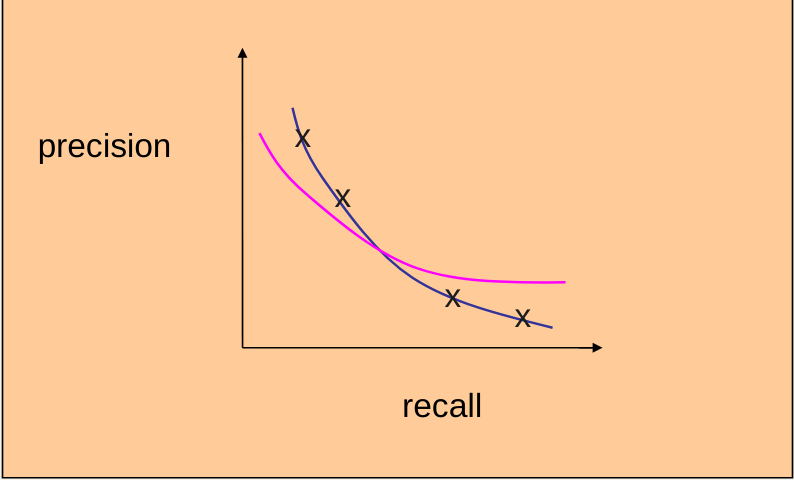
\includegraphics[width=0.7\textwidth]{Images/precisionCurve}
	\caption{Precision-Recall curve}
	\label{img:imagePrecision}
\end{figure}

      \chapter{Random Walks}
In this chapter we will consider the concept of Random Walks and also 
the evolution provided by \emph{pagerank} (invented in $1997$ by Google)
in ranking document.

Given a graph of nodes, like nodes in web graph, we use the adjacency matrix
$A$ which has $a_{ij} = 0$ if not exist a edge from $i$ to $j$ otherwise 
has value $1$.\newline
From adjacency matrix we define the transition matrix $P$, which estabilish
a weight to each edge of a graph $G$ and has as constraints that every row
in the transition matrix $P$ has to sum to $1$; in figure \ref{img:transition}
is possible to see how are defined adjacency and transition matrix for a graph,
note anyway that transition matrix is not unique.

\begin{figure}
	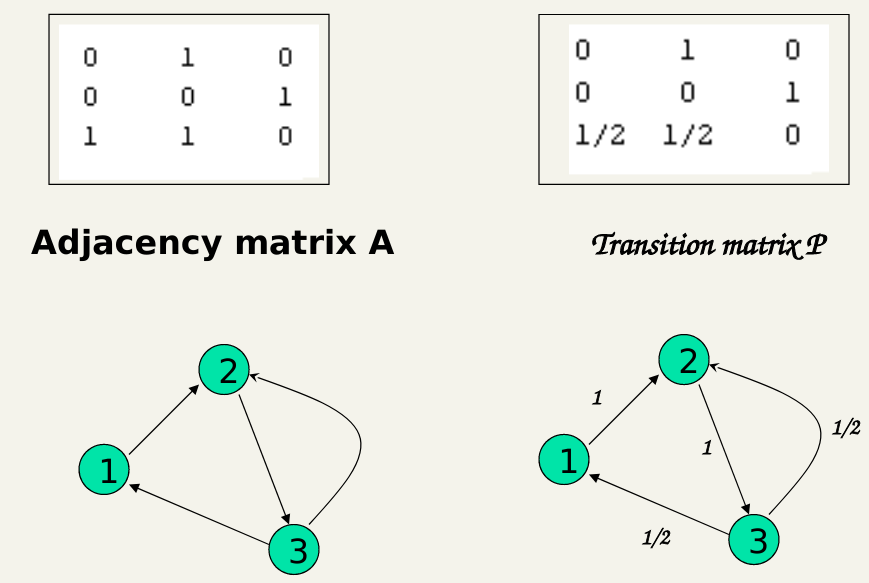
\includegraphics[width=\textwidth]{Images/transition}
	\caption{Transition matrix for a graph $G$}
	\label{img:transition}
\end{figure}
A random walk consist a random walk in the graph starting from an arbitrary
node using $t$ movement in the graph, we define the probability to be 
in a node $i$ at time $t$ as $x_t(i)$ and we update the position from time
$t$ to time $t + 1$ as 
\[ x_{t + 1}(i) = \sum _j x_t(j) * P(j, i) = x_t * P \]

Defined in that way we can obtain a recursive definition of $x_{t+1}$ as 
\[ x_{t+1} = x_t * P = (x_{t-1} * P) * P = \dots = x_0 P^{t+1} \]
If we have that the surfer keeps the same position for a long time we have
the called \emph{stationary distribution}.\newline
This distribution is related to the amound of time that a random walker
spends visiting that node and formaly is defined as 
\[ x_{t+1} = x_t \]
that corrispond to left eigenvector, with eigenvalue $1$ and for 
"well-behaved" graphs this does not depend on the start distribution $x_0$.

The stationary distribution always exist and it is unique if the graph 
(called also \emph{markov chain}) is irreducible and aperiodic, where
irreducible means that there is a path from every node to every other node
and it is aperiodic if the GCD of all cycle lengths is $1$.

\section{Link-based Ranking and Pagerank}
We view the web as a directed graph, where we have $2$ assumptions:
\begin{enumerate}
   \item A hyperlink between pages denotes author perceived relevance
	 (quality signal).
   \item The text in the anchor of the hyperlink describes the target page
	 (textual context).
\end{enumerate}


In first generation of search engine it was used link counts as simple
measures of popularity, but these approach is easy to spam, so to solve
this problem in $1997$ Google introduce \emph{Pagerank}, where each link
has its own importance and it is independent of the query.\newline
Pagerank can be viewed as a linear system of equations with billion variables
and billion contraints or also as a random walk on the Web graph, as can
be viewed in figure \ref{img:pagerank} where $\alpha = 0.85$ as google 
in the original paper estabilish.

\begin{figure}
	\includegraphics[width=\textwidth]{Images/pagerank}
	\caption{Pagerank approach on a node}
	\label{img:pagerank}
\end{figure}
Pagerank of a node is the "frequency of visit" that node by assuming an
infinite random walk and is a "measure of centrality"
of a node in a directed graph.

View a Pagerank as a linear system of equations we define the pagerank as 
\[ r(i) = \alpha * \sum _{j \in B(i)} \frac{r(j)}{\# out(j)} + 
	  (1 - \alpha) * \frac{1}{N} \]
where $\alpha = 0.85$ and $N = \#$ nodes in graph.\newline
This definition is related to the eigenvalues of the matrix 
describing the linear system of equations.

Pagerank is used in search engines in preprocessing, where given graph we
build $P$ and we compute $r = [1/N, \dots, 1/N] * P^t$, and also in 
query processing, where we retrieve pages containing query terms and 
rank them by their Pagerank.

Relevance is a not well defined mathematical concept, which is actually not 
even depending on the single user because its needs may change over time too,
so for every page search engine computes a series of features (TF-IDF, Pagerank,
occurency in URL, occurrence in the title and so on) and to rank we have
a strong use of AI and Machine Learning, using a classifier.

An evolution of Pagerank is the \emph{Personalized Pagerank}, where we bias
the random jump substituting the uniform jump to all nodes with the jump to
one specific node, which the second term is $(1 - \alpha)$ only for that node
and in the others are $0$, or a uniform jump to some set $S$ of preferred
nodes (is a generalization of the first with $|S| = 1$); it can also be 
not a uniform jump using proper weight in the definition of $r$ and the 
equation for Pagerank of a node in this personalizated version is 
\[ r(i) = \begin{cases}
	\alpha * \sum _{j \in B(i)} \frac{r(j)}{\# out(j)} + (1 - \alpha) * \frac{1}{N} \, \text{ if } i \text{ is teh personalize node } \\
	\alpha * \sum _{j \in B(i)} \frac{r(j)}{\# out(j)} \, \text{otherwise} \\
	  \end{cases} \]

\section{HITS (Hypertext Induced Topic Search}
In this section we will consider another ranking approach that has some 
pitfalls that denies his use in web engine, but are sometimes used in 
private information retrieval system.

Hits, with a common graph architecture visible in figure \ref{img:hits},
is query-dependent and produces two scores per page:
\begin{description}
    \item [Authority score:] a good authority page for a topic is pointed
	   to by many good hubs for that topic.
    \item [Hub score:] a good hub page for a topic points to many authorative
	    pages for that topic.
\end{description}

\begin{figure}
	\includegraphics[width=\textwidth]{Images/hits}
	\caption{Hits Graph architecture}
	\label{img:hits}
\end{figure}
To compute this score we have the following equations:
\begin{align*}
	a & = \transpose{A} h = \transpose{A} Aa \\
	h & = Aa = A \transpose{A} h \\
\end{align*}
where $a$ is the vector of authority's scores, $h$ is the vector of 
hub's scores and $A$ is the adjacency matrix, so we have that $h$ is an
eigenvector of $A \transpose{A}$ and $a$ is an eigenvector of $\transpose{A} A$.

We can have link with weight, so we weight more if the query occurs in the
neighborhood of the link and then we define the following equations
\begin{align*}
	h(x) & = \sum _{x \to y} w(x, y) a(y) \\
	a(x) & = \sum _{y \to x} w(x, y) h(y) \\
\end{align*}
The simple idea of rank via random walks consist to rank and select
sentences by saliency score of their constituting words $w$ computed using:
\begin{itemize}
    \item TF-IDF for weight $w$ using the formula
	    \[ saliency(S_i) = \sum _{w \in S_i} \frac{weight(w)}{|S_i|} \]
    \item Centrality over proper graphs: Pagerank, HITS, or other measures.
\end{itemize}

We introduce \emph{TextRank}, where the key issue of this approach is that 
the graph has as nodes terms or sentences and as edges the similarity 
relation between nodes defined as 
\[ Similarity(S_i, S_j) = \frac{|S_i \cap S_j}{\log |S_i| + \log |S_j|} \]
It use Pagerank over weighted graph and compute the score of nodes.

Another ranked that we will introduce is the \emph{lexical Pagerank}, which
the main difference with TextRank resides in the way it is computed 
edge weigts: it use cosine similarity via TF-IDF between sentences and 
edges are pruned if weight $<$ threshold.\newline
The scoring of nodes is done via weighted HITS to ensure mutual reinforcement
between words and sentences.

\section{LSI (Latent Semantic Indexing)}
In this section we will analyze how to reduce dimension of vector while 
we preserve distance, so to compute $cos(d, q)$ for all $n$ docs we can 
reduce the time complexity from $O(nm)$ to $O(km + kn)$ where $k << n, m$.

Instead Random projection is data-independent and consist to choose a $k$
dim subspace that guarantees good stretching properties with high probability
between any pair of points.

We will consider \emph{Latent semantic indexing}, but it can be used also
random projection, and LSI is data-dependent and it creates a $k$-dim
subspace by eliminating redundant axes and pull together hopefully 
"related" axes, like "car" and "automobile".


LSI preprocess docs using a technique from linear algebra called 
\emph{Singular Value Decomposition}, ten create a new smaller vector space
and queries are handled faster in this new space.

Recall that we have a matrix $A$ with $m \times n$ of $terms \times docs$,
so $A$ has rank $r \leq m, n$ and we define a term-term correlation matrix
\[ T = AA^T \]
that is square, symmetric $m \times m$ matrix and let $U$ be $m \times r$
matrix of $r$ eigenvectors of $T$.

In a similar way we define the doc-doc correlation matrix $D = A^t A$,
a square, symmetric $n \times n$ matrix and let $V$ be $n \times r$ matrix
of $r$ eigenvectors of $D$.

Using SVD it turns out that $A = U \Sigma V^T$, where $\Sigma$ is a diagonal
matrix with the singular values (square root of the eigenvalues of $T$) in
decreasing order.

The dimension reduction consist to fix some $k << r$ and we set all eigenvalues from $\sigma_{k+1}$ to $0$, so the new version of $\Sigma$, $\Sigma_k$ has 
rank $k$, so we can reduce the number of comparison.

$A_k$ is a pretty good approximation to $A$, since relative distances are
approximately preserved, and of all $m \times n$ matrices of rank $k$,
$A_k$ is the best approximation to $A$; to compute SVD it is required $O(nm^2)$
with $m \leq n$ but less work is required if we just want singular values, or
first $k$ singular vector or also if the matrix is sparse.

%Insert example of Projected query $q' = q V_k$

      
\end{document}
